\documentclass[conference]{IEEEtran}
\IEEEoverridecommandlockouts
% The preceding line is only needed to identify funding in the first footnote. If that is unneeded, please comment it out.
\usepackage{cite}
\usepackage{amsmath,amssymb,amsfonts}
\usepackage{textcomp}

% \usepackage[utf8]{inputenc} % allow utf-8 input
% \usepackage[T1]{fontenc}    % use 8-bit T1 fonts
\usepackage{hyperref}       % hyperlinks
\usepackage{url}            % simple URL typesetting
\usepackage{booktabs}       % professional-quality tables
\usepackage{amsfonts}       % blackboard math symbols
\usepackage{nicefrac}       % compact symbols for 1/2, etc.
\usepackage{microtype}      % microtypography
\usepackage{hyperref}
\usepackage{amsfonts}     
\usepackage{graphicx}
\usepackage{epsfig}
\usepackage{algorithm}
\usepackage{algorithmic}
\usepackage{wrapfig}
\usepackage{amsthm}
\usepackage{balance}
\usepackage{mathtools} 
\usepackage{extarrows} 
\usepackage{microtype}
\usepackage{url}
\usepackage{xcolor}
\pagestyle{empty}
%\usepackage{unicode-math}
%\setmainfont{Latin Modern Roman}
%\setmathfont{Latin Modern Math}


\newcommand{\zz}[1]{\textcolor{blue}{#1}}
\newcommand{\Xc}{{\mathcal X}}
\newcommand{\Zc}{{\mathcal Z}}
\newcommand{\Pn}{\mathbb P^{(n)}}
\newcommand{\Qn}{\mathbb Q^{(n)}}
\newcommand{\pr}{{\mathbb P}}
\newcommand{\ex}{\mathbb E}
\newtheorem{lemma}{Lemma}
\newtheorem{remark}{Remark}
\newtheorem{definition}{Definition}
\newtheorem{theorem}{Theorem}
\newcommand{\RN}[1]{%
	\textup{\lowercase\expandafter{\it \romannumeral#1}}%
}

\newcommand{\yz}[1]{{\color{red}{\bf\sf [YANG: #1]}}}


\def\BibTeX{{\rm B\kern-.05em{\sc i\kern-.025em b}\kern-.08em
    T\kern-.1667em\lower.7ex\hbox{E}\kern-.125emX}}
\begin{document}

\title{VFG: Variational Flow-Graph with Hierarchical Latent Structures\\
% \thanks{Identify applicable funding agency here. If none, delete this.}
}

\author{\IEEEauthorblockN{Anonymous submission}}

\maketitle


\begin{abstract}
This paper presents an approach to  assemble flow-based models with hierarchical structures.  With  designed  structures, the proposed model tries to uncover the latent relational structures of  high dimensional data sets.  Meanwhile, the model can generate  data representations with reduced latent dimensions, and thus it overcomes the drawbacks of many flow-based models that usually require a high dimensional latent space involving many trivial variables.  Experiments on synthetic and real world data sets show advantages and broad potentials of the proposed method. 
\end{abstract}

\begin{IEEEkeywords}
component, formatting, style, styling, insert
\end{IEEEkeywords}
\section{Introduction}
Graphical models~\cite{madigan1995bayesian,hruschka2007bayesian} synthesize the graph structure and probabilistic theory which can provide a structural probabilistic characterization of variables. Due both to the flexibility and
power of the representation and to the increased ability to effectively learn and
perform inference in large networks~\cite{koller2007graphical}, they have attracted lots of interest and been applied in many fields, \textit{e.g.} artificial intelligence like speech recognition~\cite{bilmes2005graphical}, biology like Quick Medical Reference (QMR) model ~\cite{shwe1990probabilistic} and physics like energy-based model~\cite{jordan2004graphical}.

In graphical models, we are often interested in the marginal distribution $p(\mathbf{x})$ of the observed variables $\mathbf{x}$. The maximization of such a likelihood $p(\mathbf{x})$ in a parameterized model is closely related to the inference of $p(\mathbf{x}|\mathbf{z})$ that is involved as a subroutine, given the Bayes theorem $p(\mathbf{x}|\mathbf{z}) = p(\mathbf{z}, \mathbf{x}) / p(\mathbf{x})$ where $\mathbf{z}$ is the latent variable and $p(\mathbf{x}, \mathbf{z})$ is the joint distribution. 

In this paper, we focus on this graphical inference subroutine. There are two general approaches: \textit{exact inference} and \textit{approximate inference}. $(\RN{1})$ Exact inference, \textit{e.g.} elimination algorithm~\cite{sanner2012symbolic} and junction tree algorithm~\cite{kahle2008junction}, resorts to an exact numerical calculation procedure leading to satisfactory results. However, the time complexity may be unacceptable or the intractable marginal likelihood presents a difficult challenge. Moreover, the exactitude achieved by the exact inference is not worth the computational cost in some cases, \textit{e.g.} the distribution is well determined by a small cluster of nodes in the network~\cite{jordan1999introduction}. $(\RN{2})$ In contrast, approximate inference, \textit{e.g.} Markov Chain Monte-Carlo (MCMC) and variational inference, yields deterministic approximation procedures that generally provide bounds on probabilities of interest. Considering the underlying slow convergence issues of stochastic MCMC sampling procedure~\cite{salimans2015markov}, we prefer the deterministic optimization variational inference approach to tackle with the graphical inference problem in this paper. Variational inference provides a lower bound on $p(\mathbf{x})$ and is efficiently solvable by using off-the-shelf optimization techniques, and easily applicable to large datasets~\cite{liu2016stein,kingma2013auto}.

Mean-field approximation~\cite{xing2012generalized} and variational message passing~\cite{winn2005variational} are two common approaches. They both require the intractable posterior $p(\mathbf{z}|\mathbf{x})$ that can be approximated by some family of distributions. However, on one hand, this kind of approximations is often limited by the choice of distributions that can't recover the true posterior, leading to a loose lower bound; on the other hand, they often lack a flexible structure to learn an inherent disentangled latent features thus can't encode enough information to reconstruct the data. The issues become more severe when we are dealing with higher dimensional data using a graphical model. 

Motivated by these limitations, we propose a new framework to uncover the latent relational structures of high dimensional data by crafting a variational hierarchical graphical flow model. Our contributions are threefold:
\begin{itemize}
    \item We construct hierarchical latent space between variables to uncover the latent structural relations of high dimensional data, leading to a tighter lower bound.
    \item Normalizing flow is introduced to impose a richer and tractable posterior to approximate the true posterior as the truth is more faithful posterior approximations do result in better performance.  enjoying the exact inference capability at a low computational cost.
    \item Experiments....
\end{itemize}


\section{Preliminaries}
In this section, we will first review the principles and general notations of normalizing flows and variational inference; then introduce their relations with graphical models.
\subsection{Normalizing flow}
Normalizing flow~\cite{kingma2018glow,rezende2015variational} defines an invertible transformation $f: \mathcal{Z} \xrightarrow[]{} \mathcal{X}$ between two random variables. $\mathbf{z} \sim p(\mathbf{z})$ is the latent variable which has a tractable density. $\mathbf{x} \sim p_\theta(\mathbf{x})$ is an unknown true distribution which we want to model. We usually focus on a finite sequence of transformations $f=f_1  \circ f_2   \cdot \cdot     \circ   f_L$ such that $\mathbf{x}=f(\mathbf{z})$ and $\mathbf{z}=f^{-1}(\mathbf{x})$:
\begin{align}
    \mathbf{z} \xrightleftharpoons[f_1^{-1}]{f_1} \mathbf{h}^1 \xrightleftharpoons[f_2^{-1}]{f_2} \mathbf{h}^2 \cdots \xrightleftharpoons[f_L^{-1}]{f_L}\mathbf{x}
\end{align}
Under the change of variables theorem~\eqref{eq:flow}, the probability density function~(pdf) of the model given a data point can be written as 
\begin{align}\label{eq:flow}
\log p_\theta(\mathbf{x}) =& \log p(\mathbf{z})  + \log | \text{det} ( \frac{\partial \mathbf{z} }{\partial \mathbf{x}} ) | \\
= & \log p(\mathbf{z}) + \sum_{i=1}^L\log | \text{det} ( \frac{\partial \mathbf{h}^i } {\partial \mathbf{h}^{i-1}}) | .
\end{align}
where we have $\mathbf{h}^0 = \mathbf{x}$ and $\mathbf{h}^L = \mathbf{z}$ for conciseness. The scalar value $\log |\text{det}( \frac{\partial \mathbf{h}^i}{\partial \mathbf{h}^{i-1}})|$ is the logarithm of the absolute value of the determinant of the Jacobian matrix ($\frac{\partial \mathbf{h}^i}{ \partial\mathbf{h}^{i-1}}$), also called the log-determinant. 

\subsection{Variational inference}
Given above, the mapping $f$: $\mathbf{x} \xrightarrow{} \mathbf{z}$ can be taken as encoding process (inference or recognition), and the mapping $f^{-1}$: $\mathbf{z} \xrightarrow{} \mathbf{x}$ be taken as decoding process (generation):
\begin{align}
    \mathbf{z} \sim p(\mathbf{z}), \mathbf{x} \sim p_\theta(\mathbf{x}|\mathbf{z}),
\end{align}
To learn the parameters $\theta$, one typically maximizes the following marginal log-likelihood:
\begin{align}
    \log p_\theta(\mathbf{x}) = \int p(\mathbf{z})  p_\theta(\mathbf{x}|\mathbf{z})d\mathbf{z}
\end{align}
Direct optimization of the log-likelihood is usually intractable. Variational inference instead parameterizes a family of variational distribution $q_\phi(\mathbf{z}|\mathbf{x})$ to approximate the true posterior $p_\theta(\mathbf{z}|\mathbf{x}) \varpropto  p(\mathbf{z})  p_\theta(\mathbf{x}|\mathbf{z})$, ending up optimizing the following evidence lower bound (ELBO): 
\begin{align}\label{eq:vi_elbo}
    \log p_\theta(\mathbf{x}) \geqslant \text{ELBO} &= E_{p_\theta(\mathbf{x})} 
     \{E_{q_\phi(\mathbf{z}|\mathbf{x})} \log p_\theta(\mathbf{x}|\mathbf{z}) \nonumber\\
    &\quad - \text{KL}(q_\phi(\mathbf{z}|\mathbf{x})||p(\mathbf{z}))\}
\end{align}
Since the transformation $f$ is invertible, we can simplify $q_\phi(\mathbf{z}|\mathbf{x})$ using the same set of parameters $\theta$ as in $p_\theta(\mathbf{x}|\mathbf{z})$, implying that $\phi=\theta$.

\subsection{Variational graphical models}
In directed acyclic graph models, each node $\mathbf{v}$ corresponds to a random variable, \textit{e.g.} latent variables $\mathbf{z}$ and observed variables $\mathbf{x}$ in the variational framwork and the edge represents statistical dependencies between the variables, \textit{e.g.} a function $f_\theta$ parameterized by $\theta$.  The joint distribution of the model is thus given by:
\begin{align}
    p_\theta(\mathbf{v}) = \prod_{\mathbf{v} \in \mathcal{V}} p_\theta(\mathbf{v}|pa(\mathbf{v}))
\end{align}
where $\mathbf{v}=(\mathbf{z}, \mathbf{x})$, $\mathcal{V}$ is a sample space for all graph variables and $pa(\mathbf{v})$ denotes the parent node of $\mathbf{v}$. The goal of variational Bayesian networks is to find a variational distribution, \textit{e.g.} $q(\mathbf{z}|\mathbf{x})$, to approximate the true posterior $p(\mathbf{z}|\mathbf{x})$. This exactly coincides with the general variational inference framework as in \eqref{eq:vi_elbo} in the last subsection. In this paper, we focus on the factorization of the independency of disjoint latent variables~\cite{bishop2003vibes}:
\begin{align}
    q(\mathbf{z}|\mathbf{x}) = \prod_i q_i(\mathbf{z}_i)
\end{align}
where $\mathbf{z}_i$ is the latent variable at node $i$ of the graph, implying that the observation $\mathbf{x}$ is the parent node: $\mathbf{x}=pa(\mathbf{z}_i)$. 

%%%%%%%%%%%%%%%%%%%%%%%%%%%%%%%%%%%%%%%%%%%%%%%%%%%%%%%%%%%%%%%%%%%%%%
\section{Variational Flow-Graph with Hierarchical Latent Structures}
%\yz{We need to sync the notations in the equation and the figures.}
%\yz{The ELBO should be exactly defined on the node level instead of layer level as other works have already done so~\cite{berg2018sylvester,kingma2016improved}. Will come back later when it's done}

Assume the latent space and the observation space are bridged by a sequence of variables, we can build a graphical model with normalizing flow, leading to exact latent-variable inference and log-likelihood evaluation of the model. We coin this model as \textit{Variational Flow-Graph} (VFG).
% Many real-world high dimensional datasets concentrate near low dimensional unknown manifolds. We assume the latent variables are from  a  latent space, i.e., $\mathbf{z} \in \mathbb{R}^d$, and the dimension for data sample is $D$, i.e., $\mathbf{x} \in   \mathbb{R}^D$.

\subsection{The evidence lower bound of Variational Flow-graph}
Figure~\ref{fig:node_tree} illustrates the tree structure induced by varational flow.  The hierarchical generative network has $L$ layers, and $\mathbf{h}^l$ is the latent variable in layer $l$, and $\theta$ is the parameter vector of the model. The hierarchical generative process of the model is given by 
\begin{align*}
p_\theta(\mathbf{x}) = \sum_{\mathbf{h}^1, ..., \mathbf{h}^L} p_\theta(\mathbf{h}^L)p_\theta(\mathbf{h}^{L-1} | \mathbf{h}^{L}) \cdot \cdot  \cdot  p_\theta(\mathbf{x} | \mathbf{h}^{1}) .
\end{align*}
$p_\theta(\mathbf{h}^{l-1} | \mathbf{h}^{l})$ is modeled with an invertible normalizing flow $f_\theta$. The hierarchical recognition network is factorized by
\begin{align*}
q_\theta(\mathbf{h}| \mathbf{x}) =  q_\theta(\mathbf{h}^1 | \mathbf{x})  q_\theta(\mathbf{h}^2 | \mathbf{h}^1) \cdot \cdot  \cdot  q_\theta(\mathbf{h}^{L} | \mathbf{h}^{L-1}) .
\end{align*}
where $\mathbf{h}=\{\mathbf{h}^1, \cdots, \mathbf{h}^L \}$ denotes all latent variables. 
 \begin{figure}[!htbp]
\begin{center}
 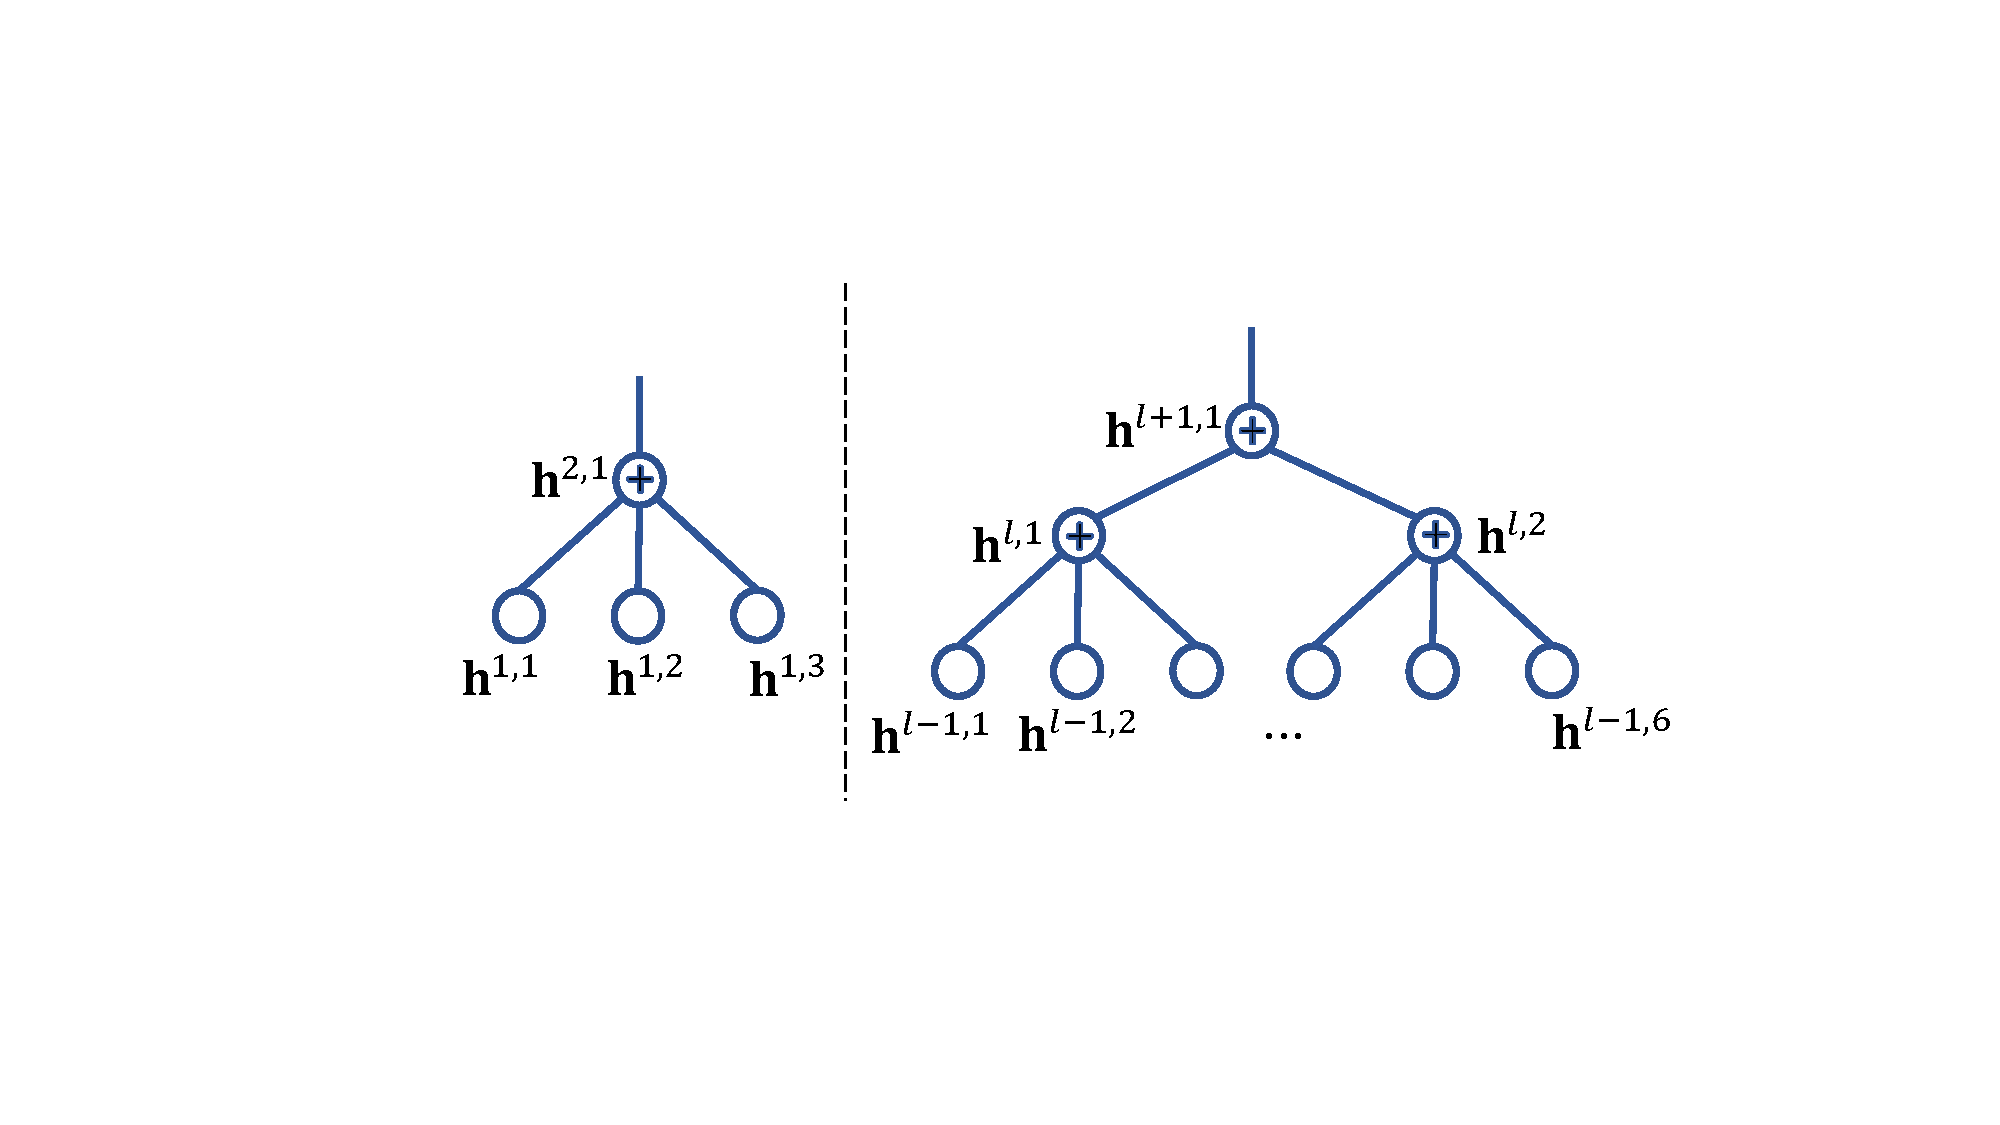
\includegraphics[width=0.95\linewidth]{fig/node.pdf}
%   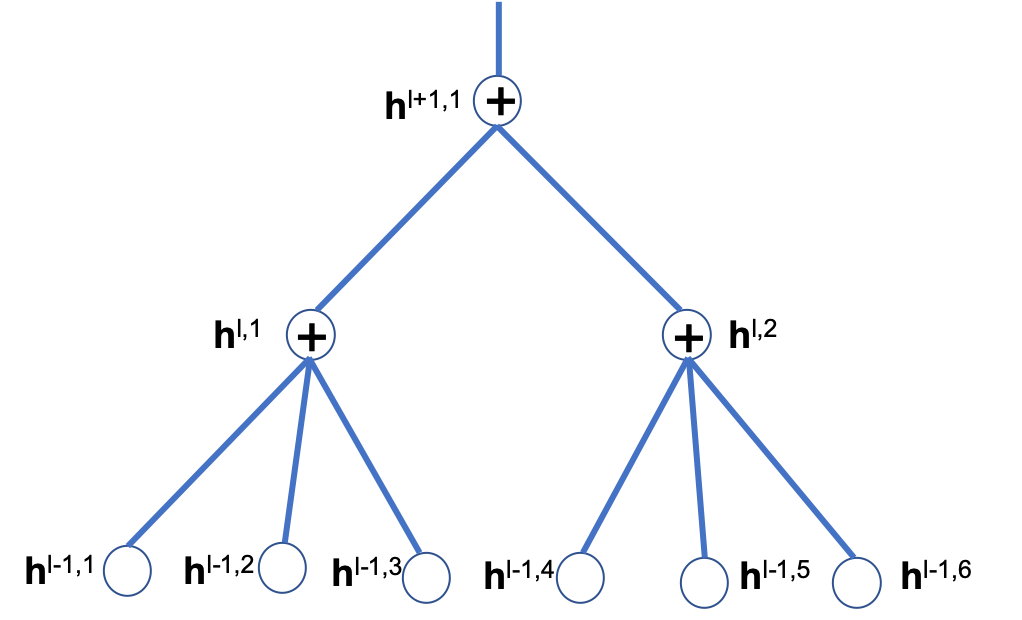
\includegraphics[width=0.55\linewidth]{fig/tree.png}
\end{center}
\caption{ (Left) The structure of one node. Node $\mathbf{h}^{2,1}$ connects with its children with invertible functions. The messages from its children are aggregated at $\mathbf{h}^{2,1}$.   (Right)An illustration of the latent structure from layer $l-1$ to $l+1$.  $\mathbf{h}^{h, i}$ means the $i$th latent variable  in layer $l$. }
\label{fig:node_tree}
\end{figure}

For node $i$, we use $\overrightarrow{\mathbf{h}}^{(i)}$ as the forward evidence message receives from its children, and $\overleftarrow{\mathbf{h}}^{(i)}$ as the  backward message from the rood. $ch(i)$ and $pa(i)$ are node $i$'s child and parent  sets, respectively.   Let $\mathbf{f}^{(j, i)}$ be the edge connecting $j$ and one of its parents $i$, and $\mathbf{f}^{-1, (j, i)}$ is its inverse function.  We have
\begin{align*}
&  \overrightarrow{\mathbf{h}}^{(i)} = \frac{1}{|ch(i)|} \sum_{j \in ch(i) } \mathbf{f}^{(j,i)}(\overrightarrow{\mathbf{h}}^{(j)}), \\ &\overleftarrow{\mathbf{h}}^{(i)} = \frac{1}{|pa(i)|} \sum_{j \in pa(i) } \mathbf{f}^{-1, (i,j)}(\overleftarrow{\mathbf{h}}^{(j)}) .
\end{align*} 
The inference procedure includes forward and backward message passings, and  the forward and backward node states are stored in these forward-backward procedures. The we can compute the layer-wise ELBO for latent states in each layer. %\textcolor{red}{More details about forward ban backward message for DAG and calculation!}
With $\mathbf{h}^0 = \mathbf{x}$, the ELBO can be derived as 
\begin{align}  \notag
& \log p(\mathbf{x}) \geqslant \mathcal{L}(\mathbf{x}; \theta) \\
& =  \sum_{l=0}^{L-1}  \mathbb{E}_{q(\mathbf{h}^{l+1}|\mathbf{h}^l)} \bigg[ \log p( \mathbf{h}^{l}|  \mathbf{h}^{l+1})   \bigg] +  \sum_{l=1}^{L-1}   \text{H}_q(\mathbf{h}^l | \mathbf{h}^{l-1} ) \nonumber \\
& \quad  -   \text{KL}\big(q(\mathbf{h}^L | \mathbf{h}^{L-1} )   | p(\mathbf{h}^L)  \big) .  \label{eq:elbo}
 \end{align}
The derivation of the ELBO can be found in the Appendix. The first term of ELBO is the reconstruction for each layer: $\mathbf{x}$ and the latent representations $\mathbf{h}^1, ..., \mathbf{h}^{L-1}$. The second and third terms are the regularizations for the latent representation. The nodes are connected with invertible functions such as flow-based models~\cite{Dinh2016DensityEU} to achieve tractable message passing. 

As shown in Figure~\ref{fig:node_tree}-(Left), a node in a flow-graph can has multiple children and multiple parents. Each node has the forward messages from the input data samples and the backward messages from the root.  If all the nodes have only one parent, then the structure is a tree. If there are nodes have multiple parents, the graph will be a DAG~(directed acyclic graph). It is easy to extend the ELBO~\eqref{eq:elbo} to DAGs with topology ordering  of the nodes and thus the layer number. We have the ELBO for a DAG structure as follows
\begin{align*}  
& \log p(\mathbf{x}) \geqslant \mathcal{L}(\mathbf{x}; \theta) \\
=&   \sum_{i \in \mathcal{G}  \setminus  \mathcal{R}_{ \mathcal{G} }  }  \mathbb{E}_{q(\mathbf{h}^{pa(i)}|\mathbf{h}^{ch(pa(i))})} \bigg[ \log p( \mathbf{h}^{(i)}|  \mathbf{h}^{pa(i)})   \bigg]  \\
 & +  \sum_{i \in \mathcal{G}  \setminus  \mathcal{R}_{ \mathcal{G} }  } H_q(\mathbf{h}^{(i)} | \mathbf{h}^{ch(i)} )   -    \sum_{i \in  \mathcal{R}_{ \mathcal{G} }  }  \text{KL}\big(q(\mathbf{h}^{(i)} | \mathbf{h}^{ch(i)} )   | p(\mathbf{h}^{(i)})  \big) .  % \label{eq:elbo}
 \end{align*}

We provide more details about the nodes in next subsection.

%The forward message comes from data samples are aggregated 
\begin{figure*}[!htbp] %{r{0.4\textwidth}
\begin{center}
 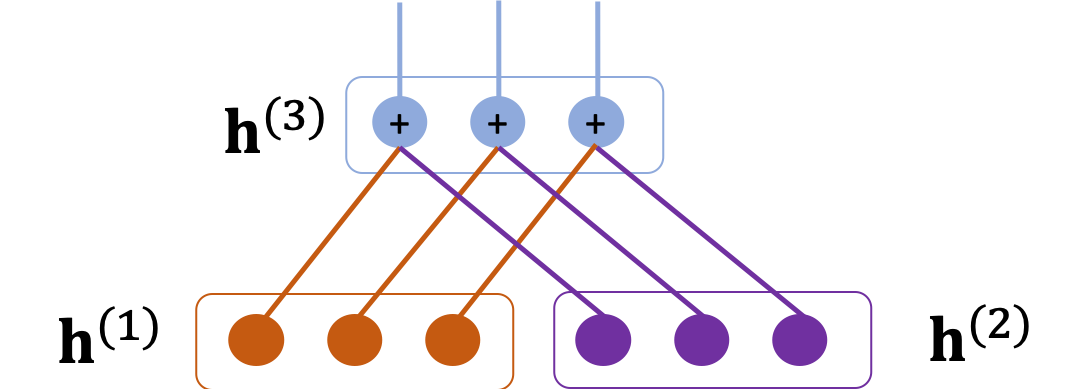
\includegraphics[width=0.43\linewidth]{fig/node_aggre_sum.png}
 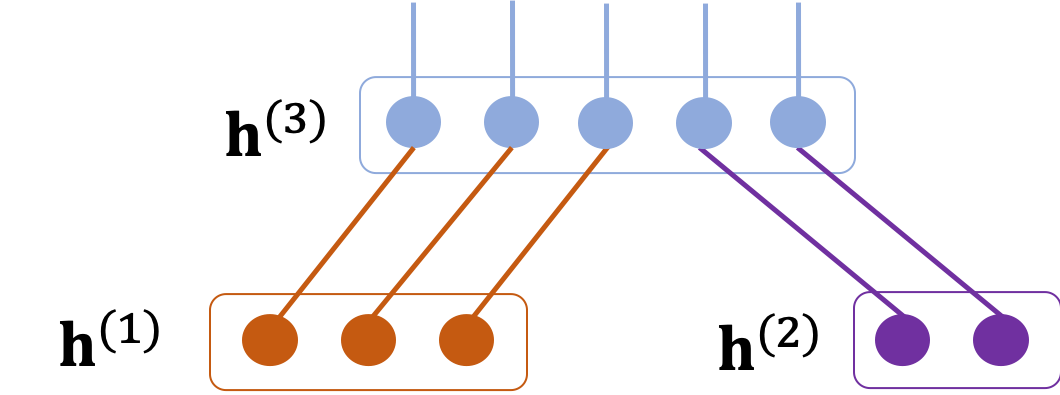
\includegraphics[width=0.43\linewidth]{fig/node_aggre_cat.png}
\end{center}
   \caption{(Left) Node aggregation with summation. (Right) Node aggregation with concatenation. }
\label{fig:node_aggre}
\end{figure*}

\subsection{Aggregation Node}
The typical prior distributions for the latent variables is Normal distribution or Uniform distribution. We use Gamma distribution as the prior for all the nodes.  It allows us to use summation operation for node aggregation.  As shown in Figure~\ref{fig:node_aggre}-left,  we assume there are link functions between  parent and the children nodes. The concatenation based node aggregation is given by Figure~\ref{fig:node_aggre}-right.

\subsubsection{Node Representation}
We assume the hidden nodes follow Normal distribution, i.e., $\mathbf{h}_j^{(i)} \sim N(k_j^{i}, \beta)$ for node $i$. $k_j^{i}$ is the shape parameter, ad $\beta$ is the scale parameter. We use the same scale parameter $\beta$ for all hidden nodes. It is easy to prove that the summation of variables follow Normal distribution follows Normal distribution as well. For a node $s$,  $j$th entry of its child $i$ follows Normal distribution,  

\subsubsection{Likelihood of Child Nodes}
The parent nodes follow Normal distribution. For a parent node $s$, the likelihood is given by 



\subsection{Inference on Sub-graphs }
\subsubsection{Inference at Single Average Aggregation Node}
%\textcolor{red}{Model it as conditional VAE problems, derive the calculation with message from the siblings.}

\begin{figure}[!htbp] %{r{0.4\textwidth}
\begin{center}
 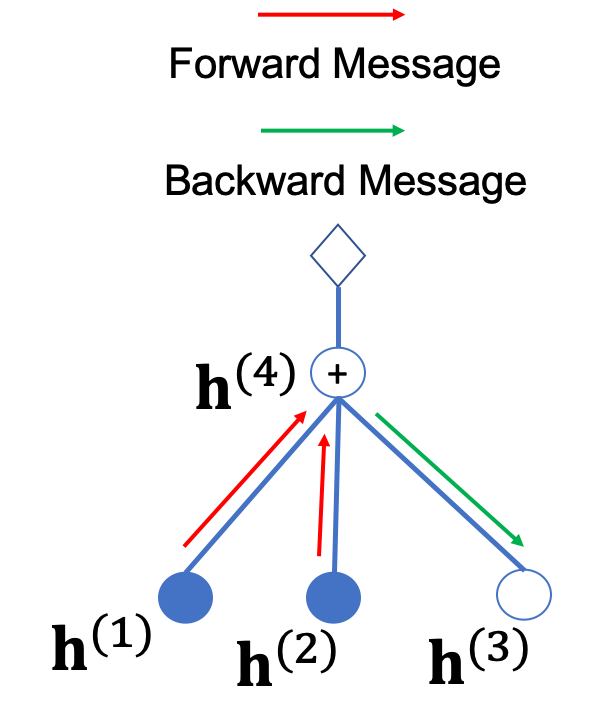
\includegraphics[width=0.43\linewidth]{fig/two_layer_infer.png}
\end{center}
   \caption{The inference of two layer model. Node 4 aggregates messages from node 1 and 2, and then pass  the updated state to node 3 for prediction.}
\label{fig:two_layer_infer}
\end{figure}

The prediction of leaf node $i$'dependents on its parents, i.e.,
\begin{align*}
p(\mathbf{h}^{(i)} | \mathbf{h}^{pa(i)}) & = p(\mathbf{h}^{pa(i)}) |\det(\frac{\partial \mathbf{h}^{pa(i)} }{\partial \mathbf{h}^{(i)}})| \\
& =
p(\mathbf{h}^{pa(i)}) |\det(\mathbf{J}^{pa(i),i})| .
\end{align*} 

The hidden state of the parent node $S$ in a bi-layer model can be approximated by the observed children
 \begin{align*}%\label{eq:gam_sum}
   \mathbf{h}^{(s)} & = \frac{1}{|ch(s)|}\sum_{i \in ch(s) \cap O} \mathbf{h}^{(i)} 
 \end{align*}
 
 Here $O$ is the set of observed leaf nodes. Figure~\ref{fig:two_layer_infer} illustrates one example of the bi-layer  case. 

\begin{figure}[!htbp] %{r{0.4\textwidth}
\begin{center}
 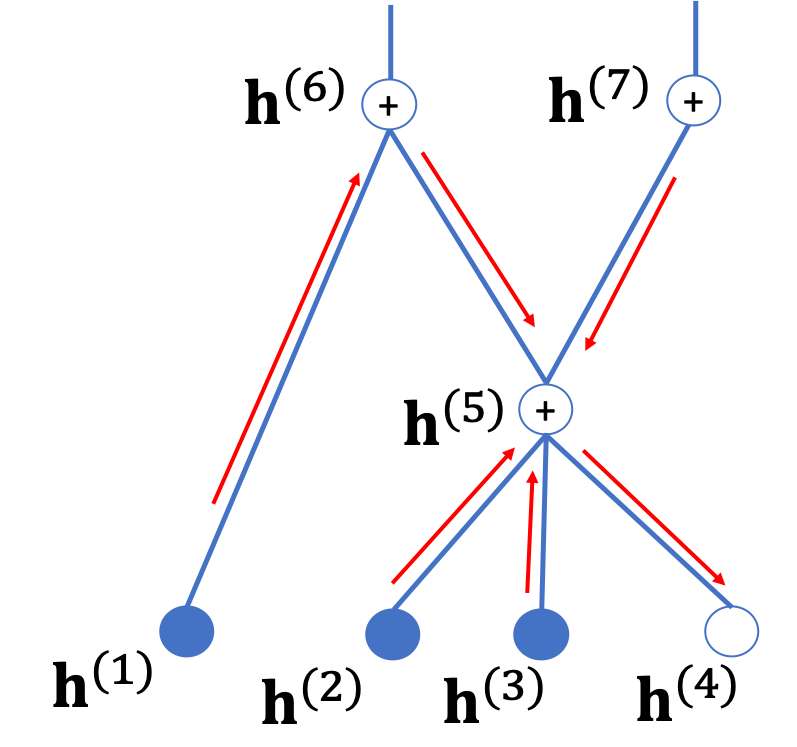
\includegraphics[width=0.43\linewidth]{fig/dag_infer.png}
\end{center}
   \caption{The inference on a DAG model. Observed node states are gathered in node 5 to predict the state of node 4. }
\label{fig:dag_infer}
\end{figure}

For a node in a DAG model, its state is updated with messages from its children's updating and then pass it to   children without updating. Figure~

\begin{lemma}
The highest node involved in  inference is the highest co-ancestor of the observed  and  missing nodes.
\end{lemma}





\subsubsection{Recover the Data Structure Based Tree and DAG}


We use the Jacobian matrix to evalue the relationship between variables. According to the change of variable rule, $p(\mathbf{x}) = p(\mathbf{z})|\det\big(\frac{\partial \mathbf{z}}{\partial \mathbf{x}}\big)|$. There are two Jacobian metrics for a flow-graph model that are obtained in the forward and backward passage passings respectively.  

With $\overleftarrow{\mathbf{J}} = \frac{\partial \mathbf{x}}{\partial \mathbf{z}}$ and  $\overrightarrow{\mathbf{J}} = \frac{\partial \mathbf{z}}{\partial \mathbf{x}}$, we use the following matrix to determine the relation between entries of $\mathbf{x}$,
\begin{align*}
\mathbb{E}_{\mathbf{x} \sim D} \big[
\overleftarrow{\mathbf{J}}
\overrightarrow{\mathbf{J}}  \big] .
\end{align*}

For a tree structure, we use $\overleftarrow{\mathbf{J}}= \frac{\partial \mathbf{x}}{\partial \mathbf{h}^{L}}$, and $\overrightarrow{\mathbf{J}}  = \frac{\partial  \mathbf{h}^{L} }{\partial \mathbf{x} }$, and we have a similar result.
\begin{align} \label{eq:Jfb}
\overrightarrow{\mathbf{J}} = \Pi_{i=1}^L\overrightarrow{\mathbf{J}^l} , \ 
\overleftarrow{\mathbf{J}} = \Pi_{i=1}^L\overleftarrow{\mathbf{J}^l}  .
\end{align}

In a DAG model, the forward and backward Jacobian is computed in a similar approach in~\eqref{eq:Jfb}, but with $L$ as the level number of topology layer. For a node  $i$,
\begin{align*}
&  \overrightarrow{\mathbf{J}}^{(i)} = \frac{1}{|ch(i)|} \sum_{j \in ch(i) } \mathbf{J}^{(i,j)}, \\ &\overleftarrow{\mathbf{J}}^{(i)} = \frac{1}{|pa(i)|} \sum_{j \in pa(i) } \mathbf{J}{(j,i)} .
\end{align*} 
In topology layer $i$, $ \overrightarrow{\mathbf{J}}^{l}$ is the concatenation of the Jocobians regarding its children, and  $ \overrightarrow{\mathbf{J}}^{l}$ is the concatenation of the Jocobians regarding its parents. 


\subsubsection{Prediction with Partial Observed Data}

The tree and DAG structures enable the model to perform message passing  among the nodes. The model can perform data imputation with partial observed data as the input. We also can use the model for multi-modal data integration and prediction.  These applications rely on effective message passing among the node. Let's assume each data sample consist $m$ sections, $\mathbf{x} = \{ \mathbf{x}_1,  \mathbf{x}_2, ..., \mathbf{x}_m \}$, then we have the following lemma regarding the model.

\begin{figure*}[!htbp]%{r{0.4\textwidth}
\begin{center}
 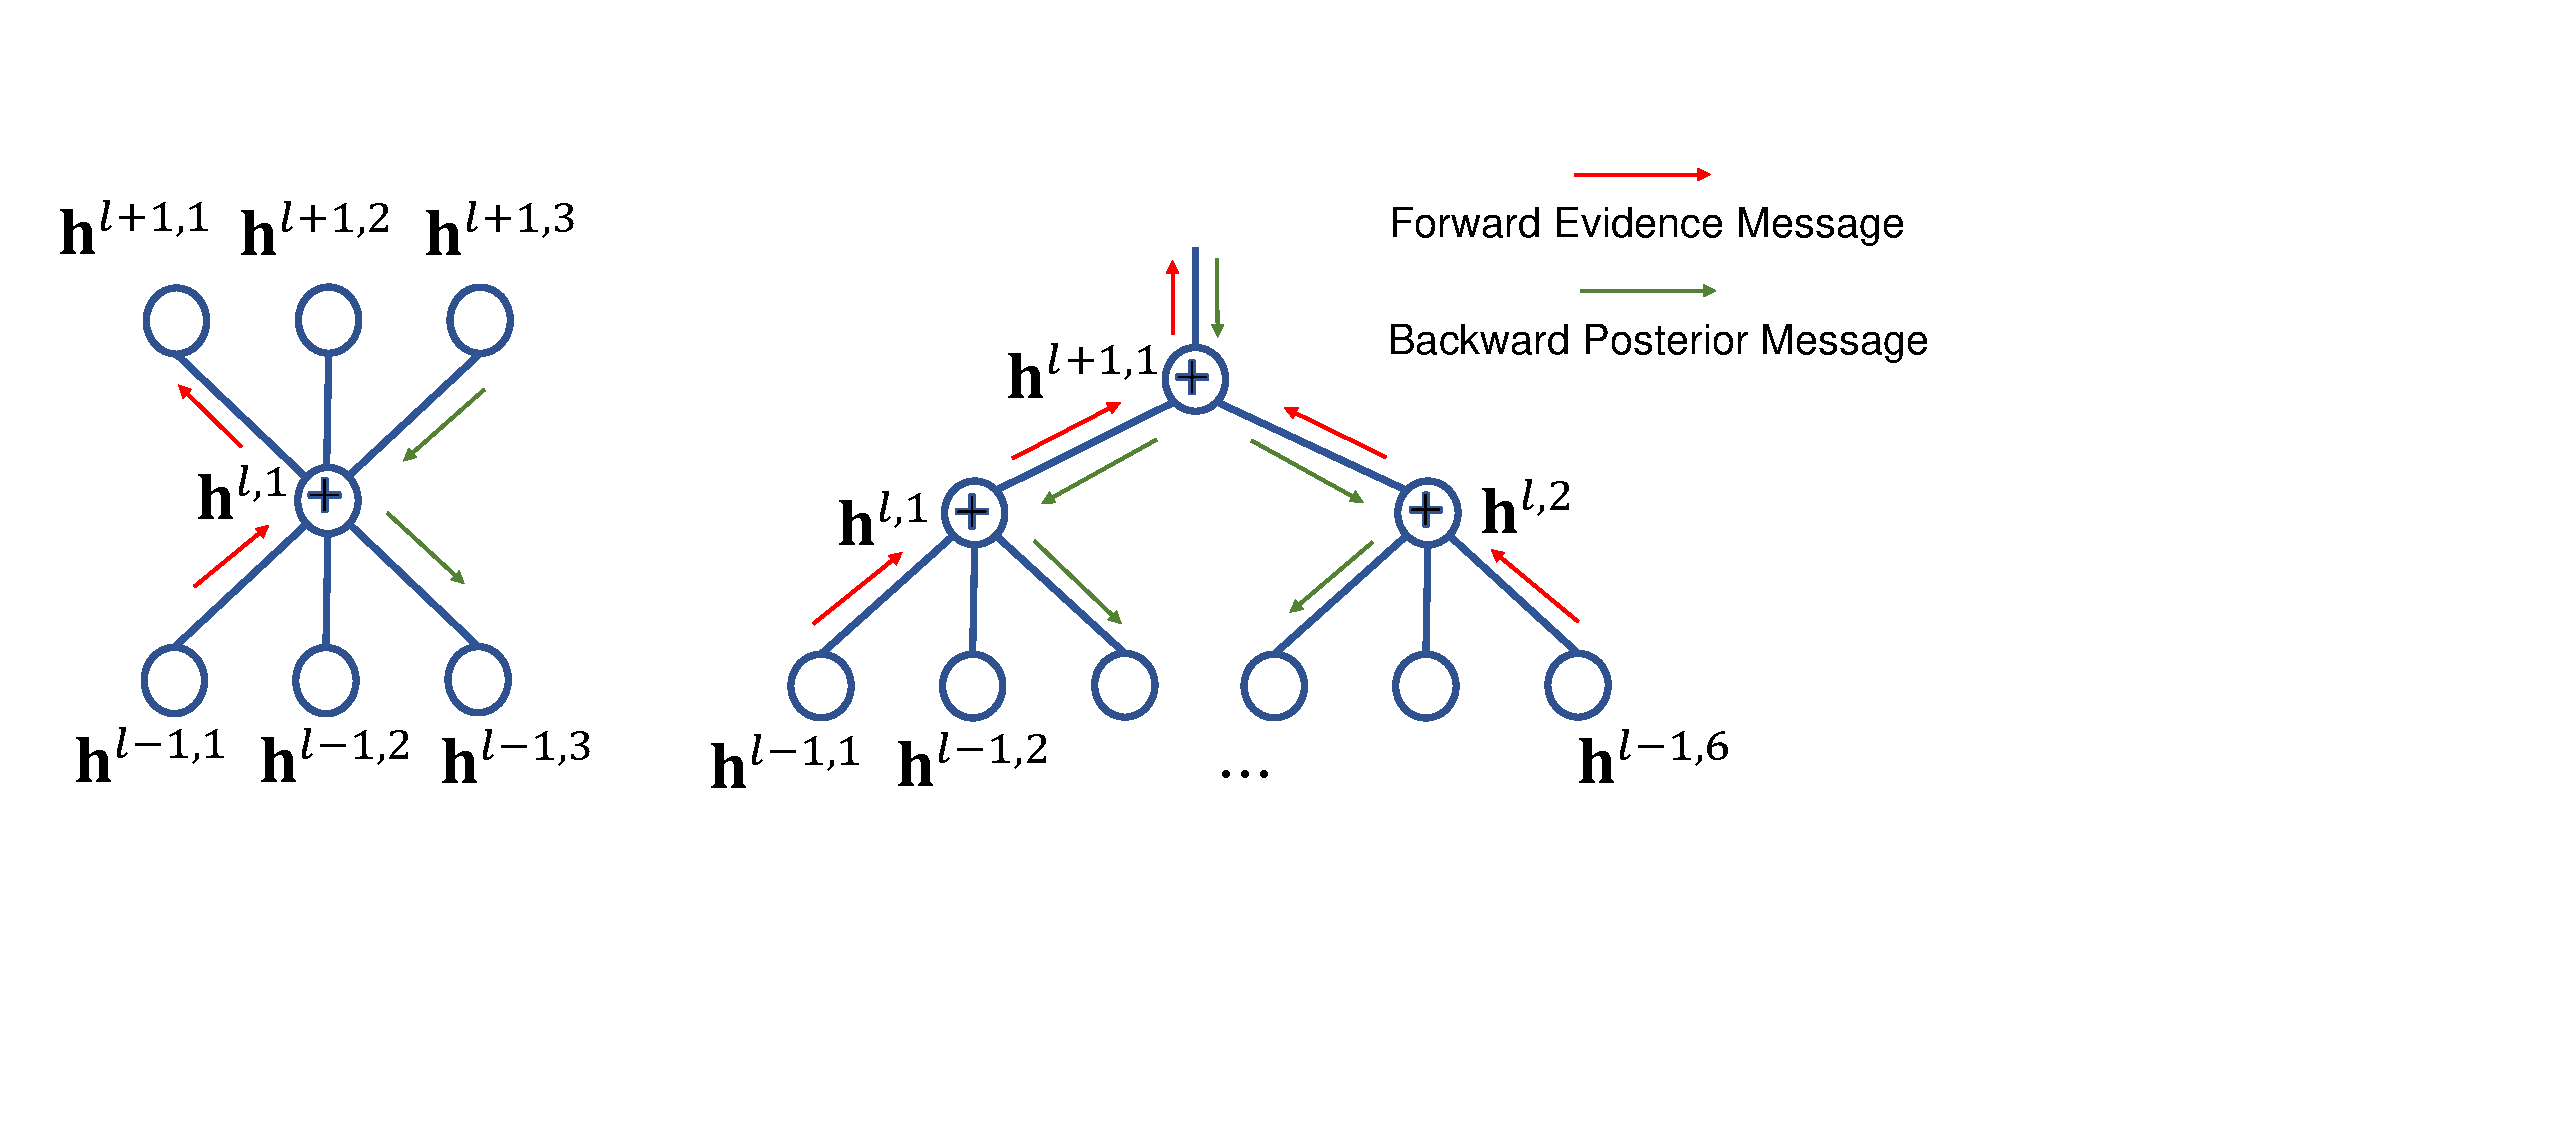
\includegraphics[width=0.6\linewidth]{fig/message_pass.pdf}
   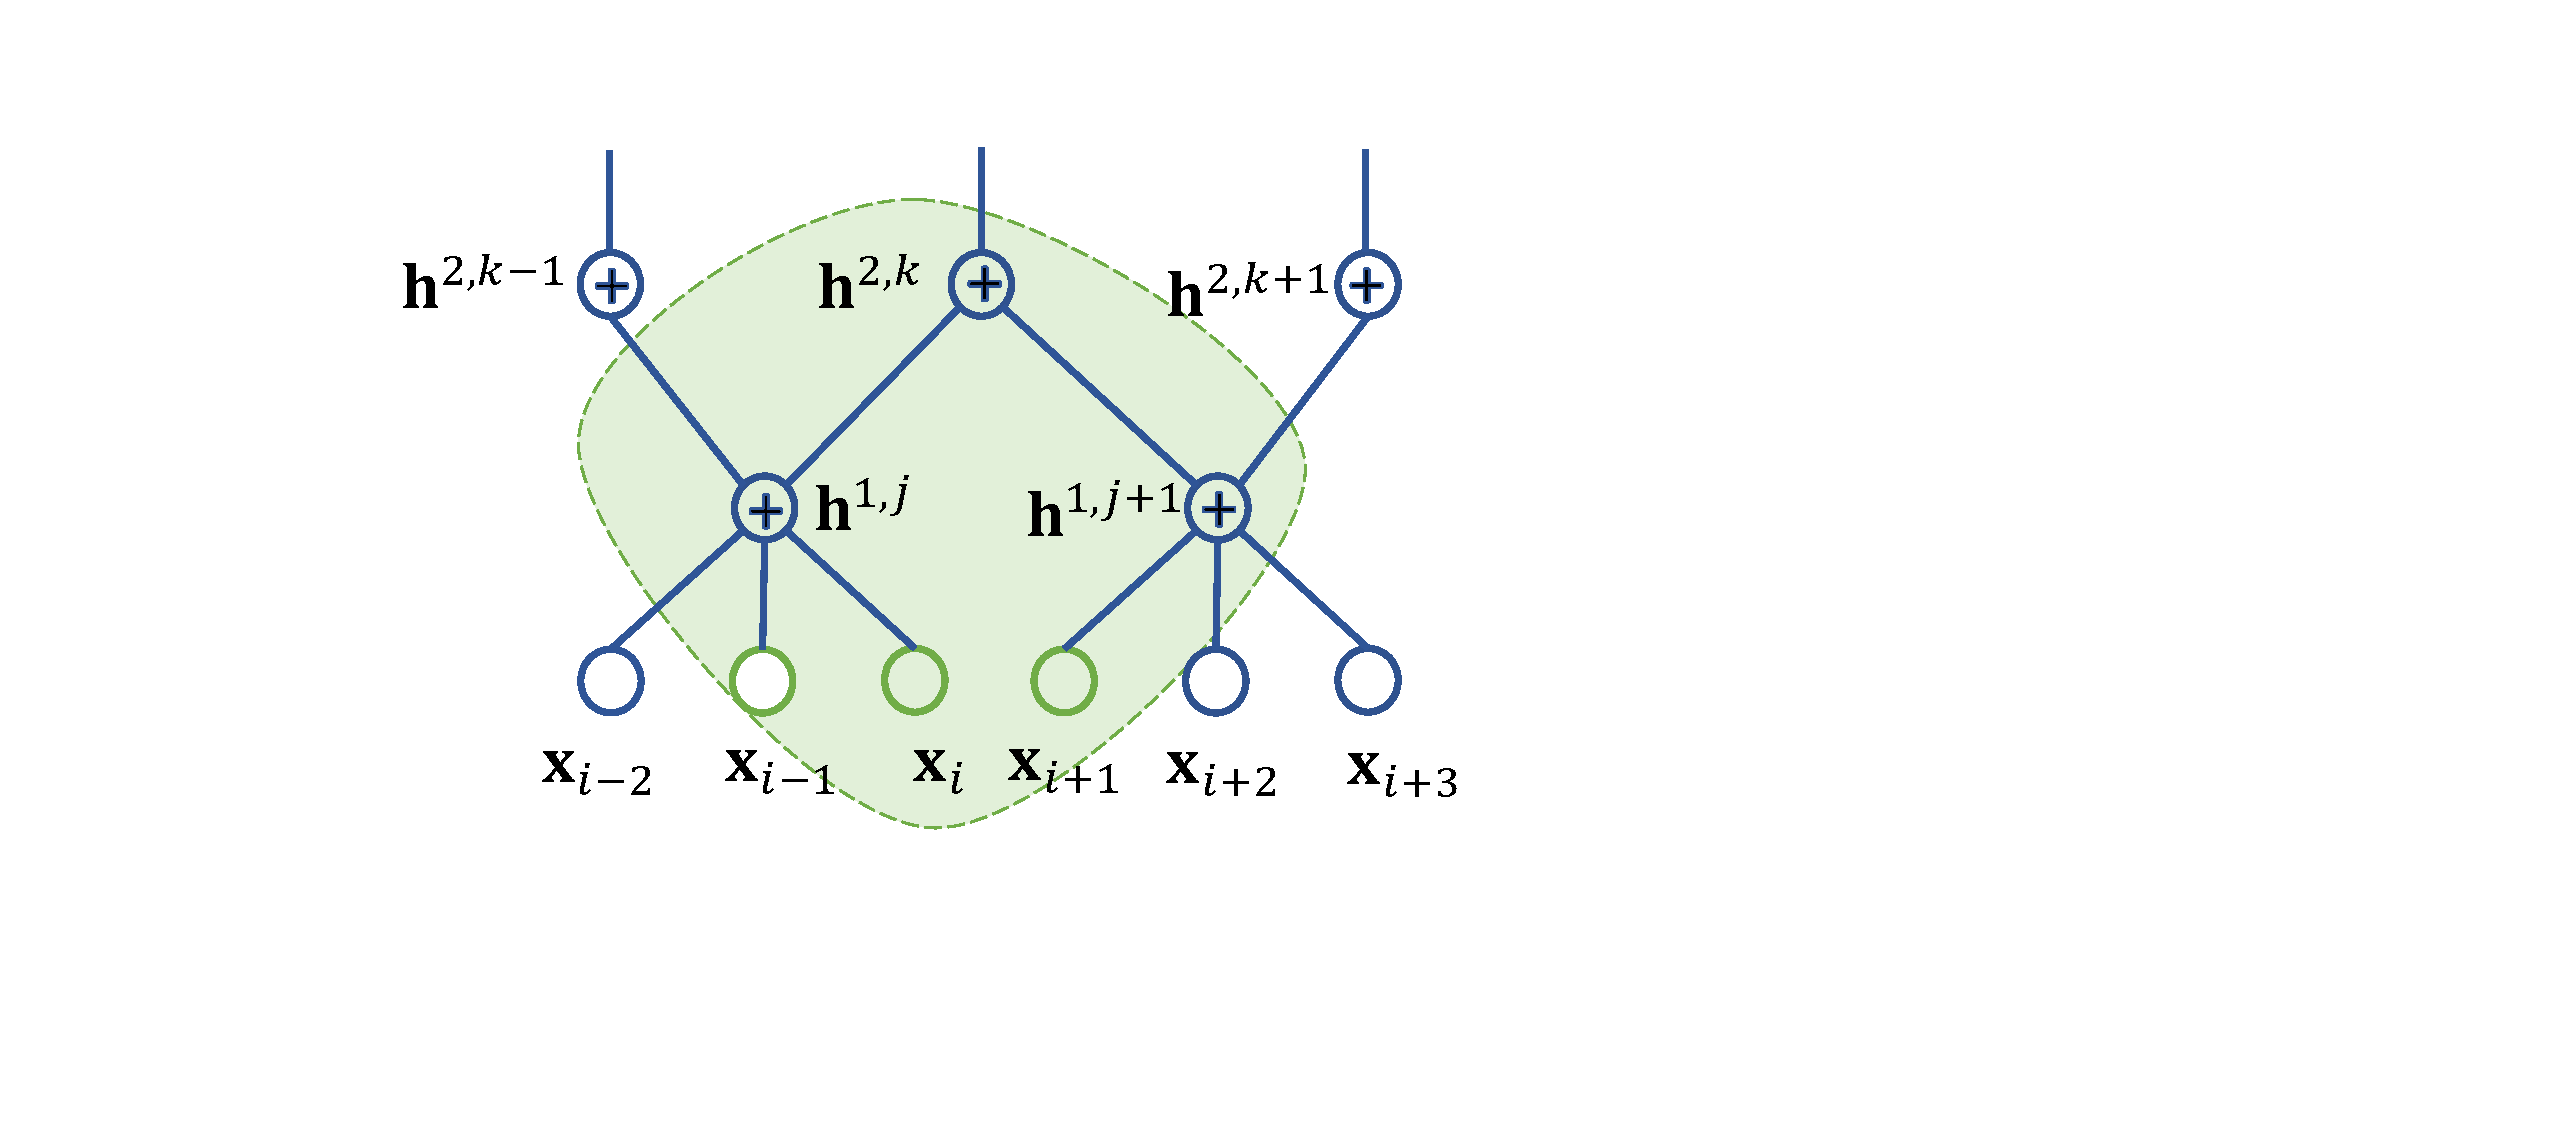
\includegraphics[width=0.35\linewidth]{fig/markov_blanket.pdf}

\end{center}
   \caption{(Left) Message passing in a node. (Middle) Message passing in a tree. (Right) Markov blanket of node $\mathbf{x}_i$. In this example, $\mathbf{x}_i$ correlates with data sections $\mathbf{x}_{i-1}$ and  $\mathbf{x}_{i+1}$.   }
\label{fig:mblanket}
\end{figure*}

Given a set of data with multiple sections, we cannot directly recover the structural relations among these sections. However, we have the following lemma regarding the latent structure.


\begin{lemma}
Let $\mathcal{S}(i)$ be the set of data sections correlate section $i$, then the Markov blanket of node $i$ is the  Markov blanket  of   $\mathcal{S}(i) \cup \{i\}$ recovered by the model. 
\end{lemma}

\begin{proof}
As  the nodes in $\mathcal{S}(i) \cup \{i\}$ do not have child nodes, we only consider the patient nodes. It is easy to see that with the penalty term in objective~\eqref{eq:objective} always lead to a smaller loss value if $\mathbf{f}^{(i,k)}(\mathbf{x}_i)$ is approximate with the messages from the the nodes in the Markov blanket of $\mathcal{S}(i) \cup \{i\}$ . 
\end{proof}


\subsection{Hierarchy Disentanglement with Flow-Graph}

Experiments on MNIST data set. A picture to show the hierarchy structure. 

\subsection{Algorithm and Implementation}

\subsubsection{Algorithms}
The model parameters for  flow graph can be learning with likelihood maximum.  For each node,  we have to ensure the  inputs from multiple edges are as close as possible.  To train the graph, we first apply forward propagation to get the latent variable $\mathbf{z}$, and then layer-wisely train each layer with likelihood back-propagation. 

\begin{algorithm}[h!]
   \caption{Inference model parameters with layer wise forward and backward message propagation}
   \label{alg:main}
\begin{algorithmic}
   \STATE {\bfseries Input:} Data distribution $\mathcal{D}$,  $\mathcal{G} = \{\mathcal{V}, \mathbf{f}\}$
   \REPEAT
   \STATE Sample minibatch $b$ samples $\{\mathbf{x}_1, ..., \mathbf{x}_b \}$ from $\mathcal{D}$;
   \FOR{$i \in \mathcal{V}$}
   \STATE $\overrightarrow{\mathbf{h}}^{(i)} = \frac{1}{|ch(i)|} \sum_{j \in ch(i) } \mathbf{f}^{(j,i)}(\overrightarrow{\mathbf{h}}^{(j)})$; \\ \textcolor{blue}{// forward message passing}
   \ENDFOR
    \STATE  $ \overrightarrow{\mathbf{h}} =  \{\overrightarrow{\mathbf{h}}^{(1)}, ...,  \overrightarrow{\mathbf{h}}^{(|\mathcal{V}|)}  \}$;
    \FOR{$i \in \mathcal{V}$}
   \STATE $\overleftarrow{\mathbf{h}}^{(i)} = \frac{1}{|pa(i)|} \sum_{j \in pa(i) } \mathbf{f}^{-1, (i,j)}(\overleftarrow{\mathbf{h}}^{(j)}) $; \\ \textcolor{blue}{// backward message passing}
   \ENDFOR
    \STATE  $ \overleftarrow{\mathbf{h}} =  \{\overleftarrow{\mathbf{h}}^{1}, ...,  \overleftarrow{\mathbf{h}}^{(|\mathcal{V}|)}  \}$;
    
    \STATE Updating flow-graph $\mathcal{G}$ by descending the gradient $\bigtriangledown_{\theta_{\mathbf{f}}}\frac{1}{b} \sum_{i=1}^b  \big[ -\mathcal{L}(\mathbf{x}; \theta_{\mathbf{f}} ) +\lambda \Psi(\mathbf{x}; \theta_{\mathbf{f}}) \big] $ ;
   %\ENDFOR 
   \UNTIL{Converge}
\end{algorithmic}
\end{algorithm}



\subsubsection{Implementation Details}

The nodes are connected with flow-based models. Different from VAE~\cite{kingma2013auto}, variational flow-graph~(VFG) uses the same network for both encoding and decoding. We assume the latent variables are following Gaussian distribution. We use the empirical variance as the conditional variance to compute the entropy and KL terms. Besides the aggregation nodes, we also use concatenation nodes to increase the flexibility of the structure. Each node can use part of its variables to connect with its parents. 

%\textcolor{red}{need a lemma here}

\section{Experiments}

\subsection{Metrics}
The data set is divided into training and testing sets. The model is trained with the training set, then it is used to infer the missing entries of samples in the testing set.

\subsubsection{Imputation}

We use the following baselines for data imputation.

\begin{itemize}
\item \textbf{Mean Value} \ We can directly use the mean values in the corresponding position of training set to replace the missing entries in the testing set.  

\item \textbf{Iterative Imputation} A strategy for imputing missing values by modeling each feature with missing values as a function of other features in a Round-Robin fashion. We choose the KNeighborRegressor as the specific function~\cite{scikit-learn}.

\item \textbf{KNN} \  To use K-Nearest Neighbor for data imputation,  we compare the non-missing entries of each sample to the training set and use the  average of top $k$ samples to impute the missing entries. 

\item \textbf{Multivariate Imputation by Chained Equation (MICE)} \ This method impute the missing entries with multiple  rounds of inference. The method can handle different kind data types.
\end{itemize}

\subsection{Evaluation with Synthetic  Data  }
In this set of experiments, we study the proposed model with synthetic data sets.
We use two latent variables, i.e. Z

We generate 1000 data points for model training, and each data sample  has 8 dimension with 2 latent variables.  The relation between the latent variables and the 

\subsubsection{Likelihood Testing}

The data is generated according to $\mathbf{x} = []$. 

Figure~\ref{fig:elbo} gives the likelihood value of the proposed method. 

\begin{figure}[!htbp]
    \centering
    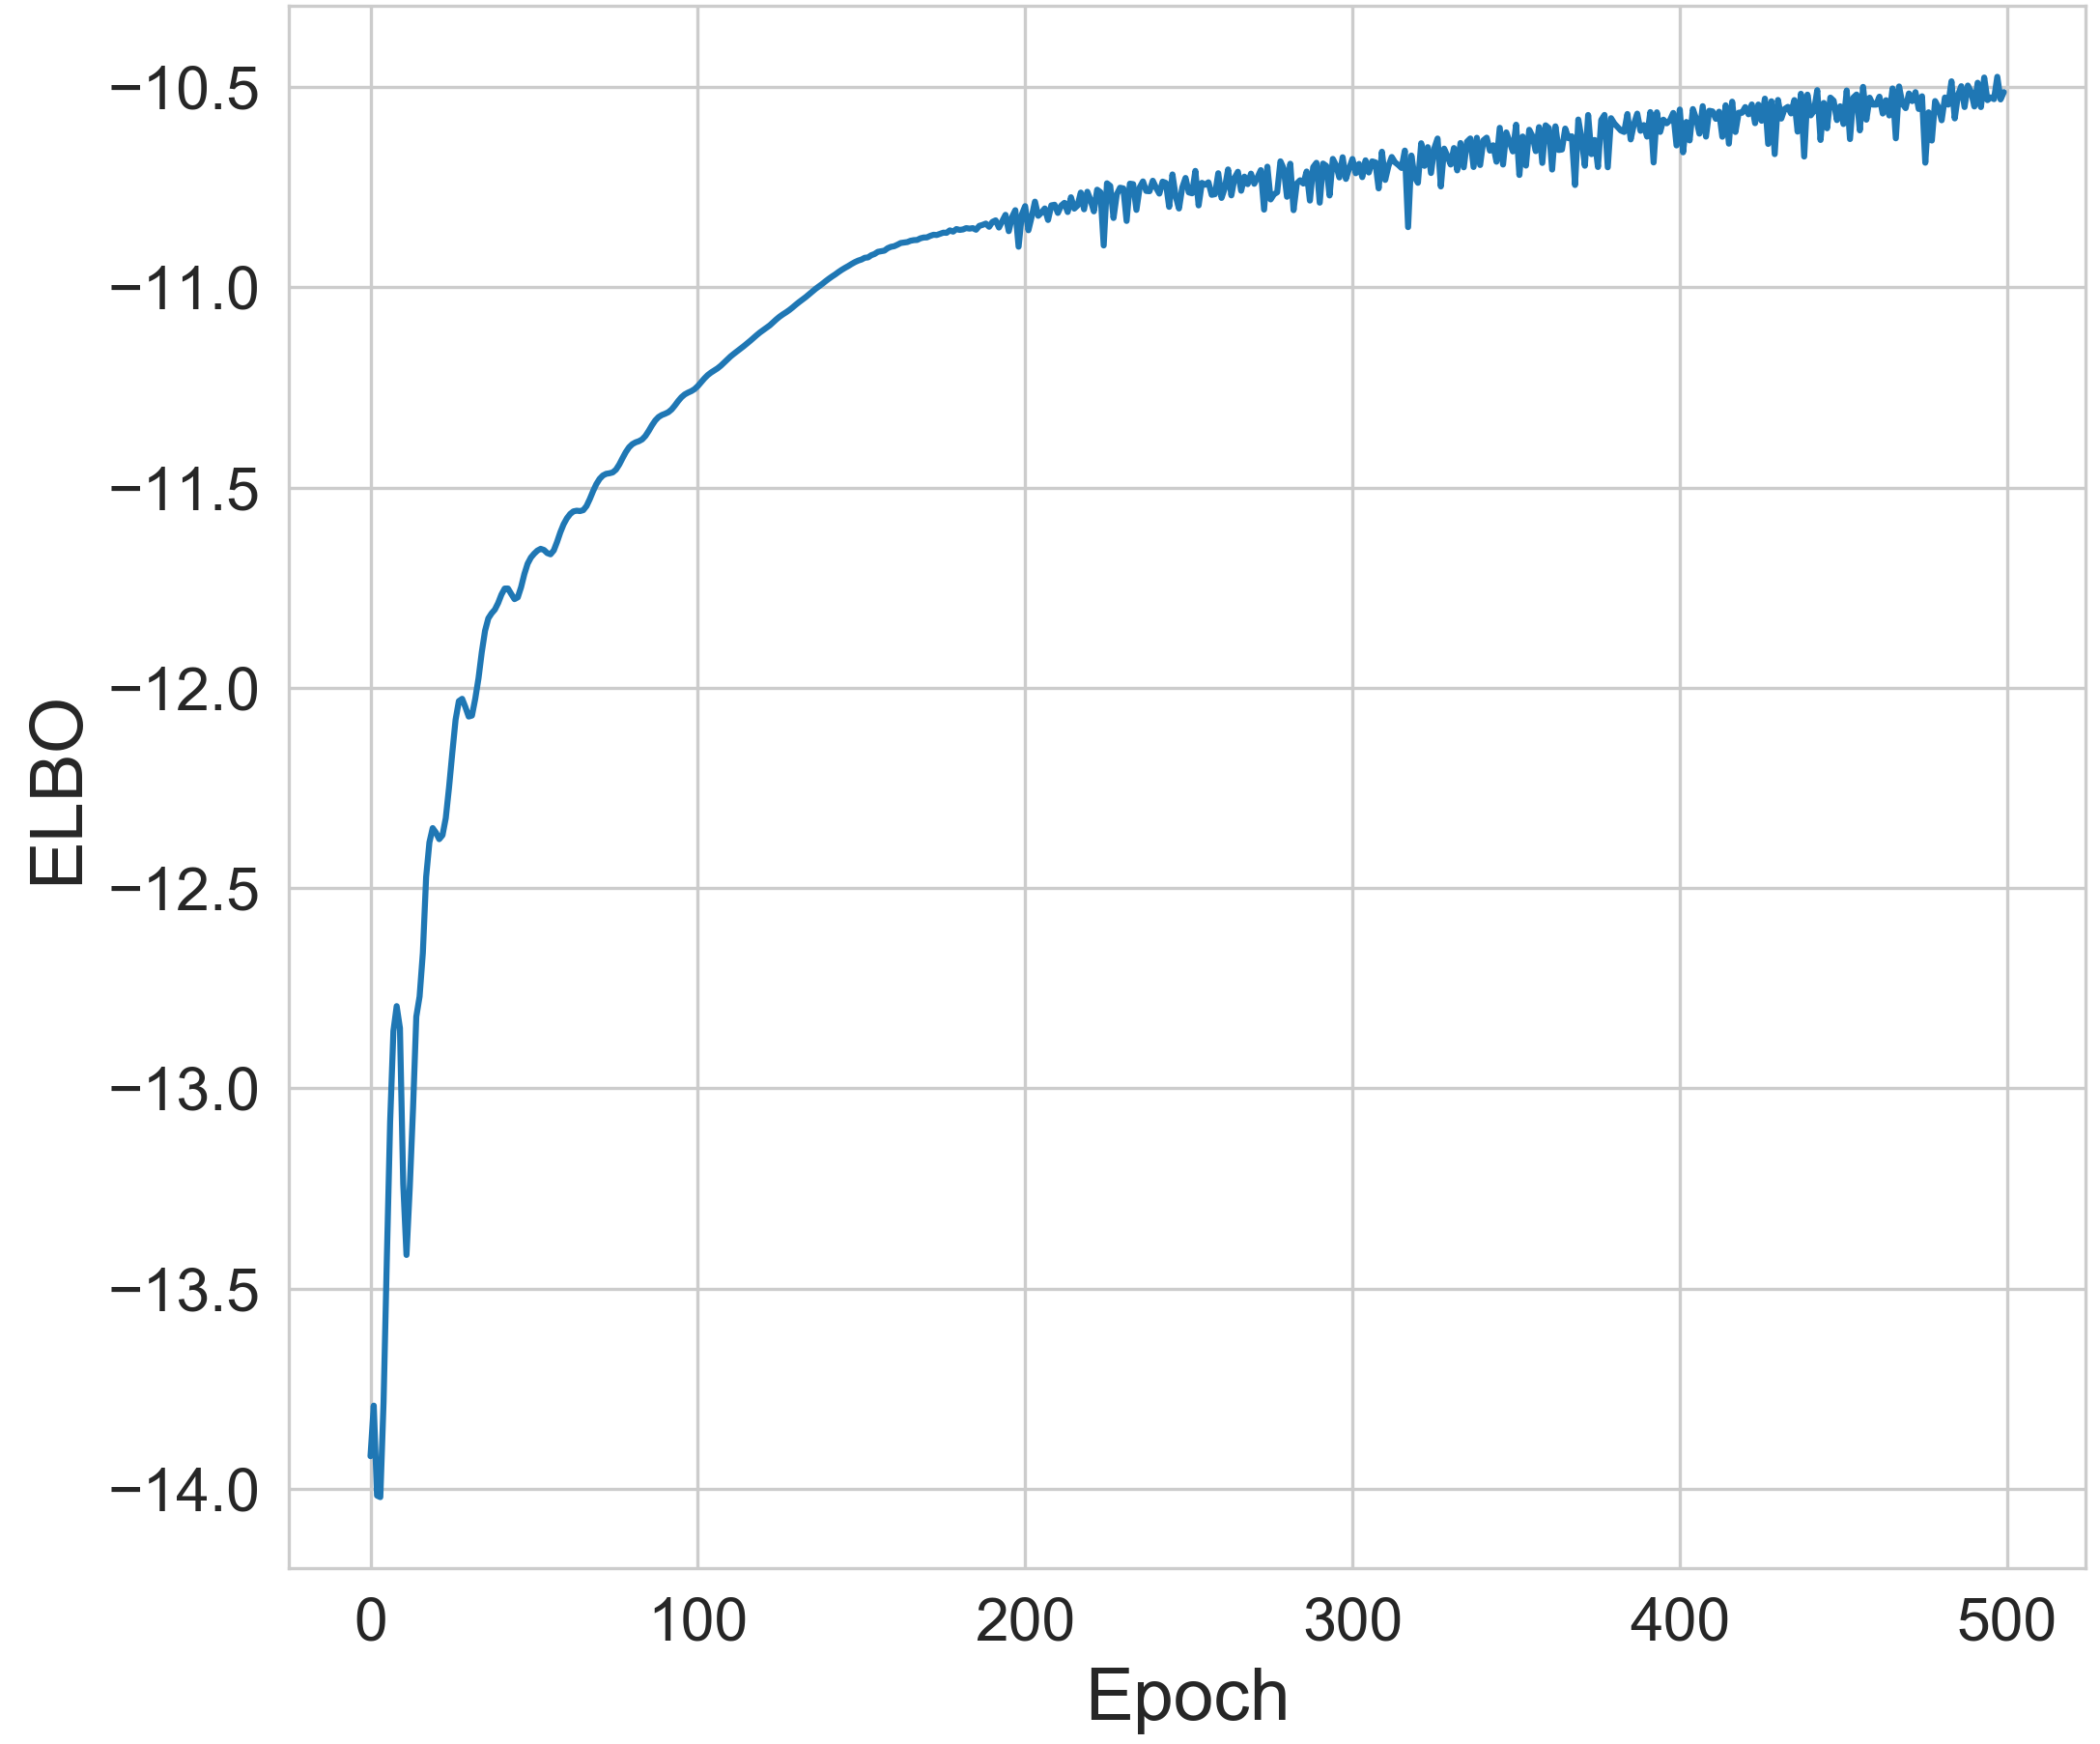
\includegraphics[width=2.3in]{fig/elbo.png}
    \caption{ELBO on the synthetic data}
    \label{fig:elbo}
\end{figure}

\begin{figure*}[!htbp]
    \centering
    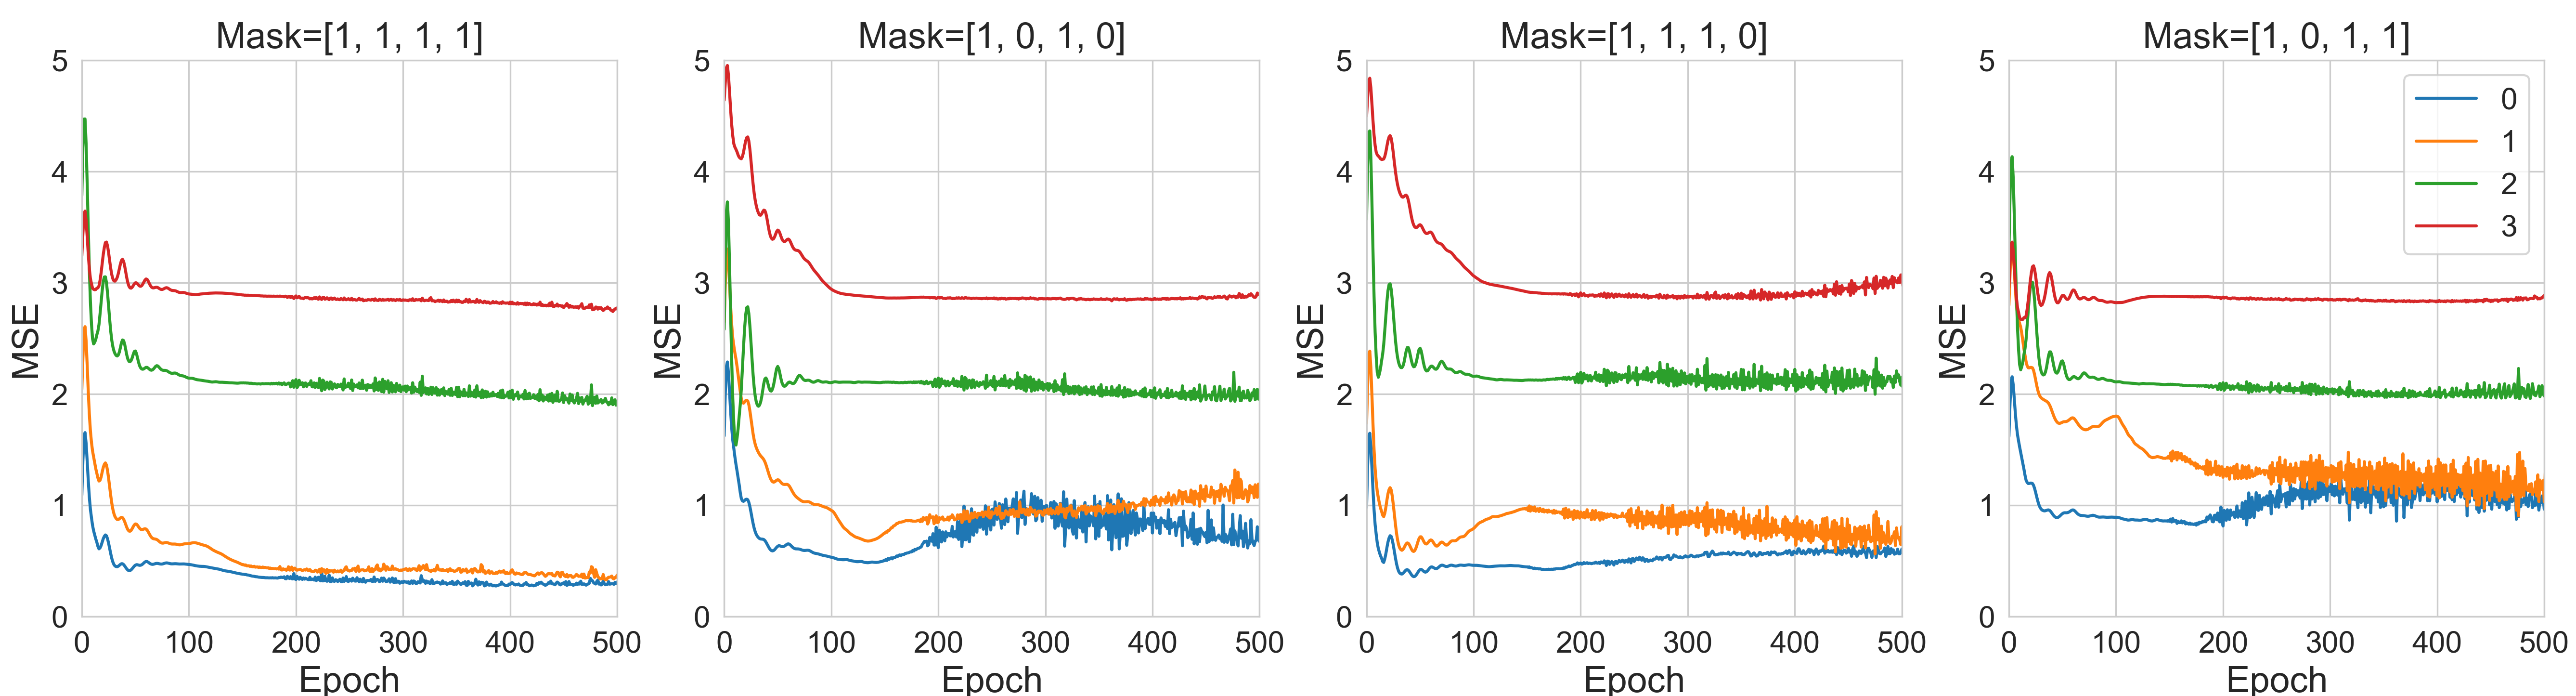
\includegraphics[width=0.95\textwidth]{fig/mse.png}
    \caption{Imputation with $\mathsf{Mask}$ on the child nodes [0, 1, 2, 3] indicated by colored legends. }
    \label{fig:mse}
\end{figure*}

\subsubsection{Data Imputation}

%\subsubsection{Graph Structure Recovery}
\begin{table}[t!]
\begin{center}
%\vspace{0.15in}
\caption{Imputation Results on Synthetic Data.} \label{tab:causality2}
\begin{tabular}{l | c  }\hline
Methods & Imputation MSE  \\
\hline
Mean Value &8.43 \\
\hline
MICE &8.38 \\
\hline
Iterative Imputation & 2.64 \\
\hline
KNN (k=3) &0.14 \\
\hline
KNN (k=5) &0.18 \\
\hline
Proposed &  1.45  \\  
\hline
\end{tabular}
\end{center}
\end{table}



\subsection{Imputation on Real-World Data Sets}

\subsubsection{Arrhythmia Data Set}
We further investigate the method on a tabular data set.  The Arrhythmia~\cite{Dua:2019}  data set is  obtained from the ODDS repository. The smallest classes, including 3, 4, 5, 7, 8, 9, 14, and 15, are combined to form the anomaly class, and the rest of the classes are combined to form the normal class. Table 4 shows the anomaly detection results with different methods. 


% Due to the small training set, classic methods outperform  deep generative models on precision and F1 score.  However, our method achieves the highest recall values and a high F1 score as well. With the help of the variance network, our method is relatively robust compared with other deep neural network methods. More details about the implementation  of the InvGAN can be found in Appendix B. Figure 5 gives the convergence of the loss $L_{h,\sigma}$ for different data sets. %



\subsection{Structured Data}
\subsubsection{Graph}

%\subsubsection{Structure Learning}

\section*{Acknowledgment}

The preferred spelling of the word ``acknowledgment'' in America is without 
an ``e'' after the ``g''. Avoid the stilted expression ``one of us (R. B. 
G.) thanks $\ldots$''. Instead, try ``R. B. G. thanks$\ldots$''. Put sponsor 
acknowledgments in the unnumbered footnote on the first page.

\bibliographystyle{IEEEtranS}
\bibliography{IEEEabrv,ref}

\clearpage
\section*{Appendix A.  ELBO of Tree Models}\label{appd:tree_elbo}

The hierarchy generative network as given in Figure~\ref{fig:tree-d}. For each pair of connected nodes, the edge is linked with an invertible function. We use $\theta$ to represent the parameters for all the edges.
The forward message passing starts from $\mathbf{x}$ and ends at $\mathbf{h}^L$, and backward message passing is in the reverse direction. 
 Then the
 likelihood for the data is given by
\begin{align*}
p(\mathbf{x}| \mathbf{\theta}) = \sum_{\mathbf{h}^1, ..., \mathbf{h}^L} p(\mathbf{h}^L | \theta)p(\mathbf{h}^{L-1} | \mathbf{h}^{L},\theta) \cdot \cdot  \cdot  p(\mathbf{x} | \mathbf{h}^{1}, \theta) .
\end{align*}

\begin{figure}[!htbp]
    \centering
    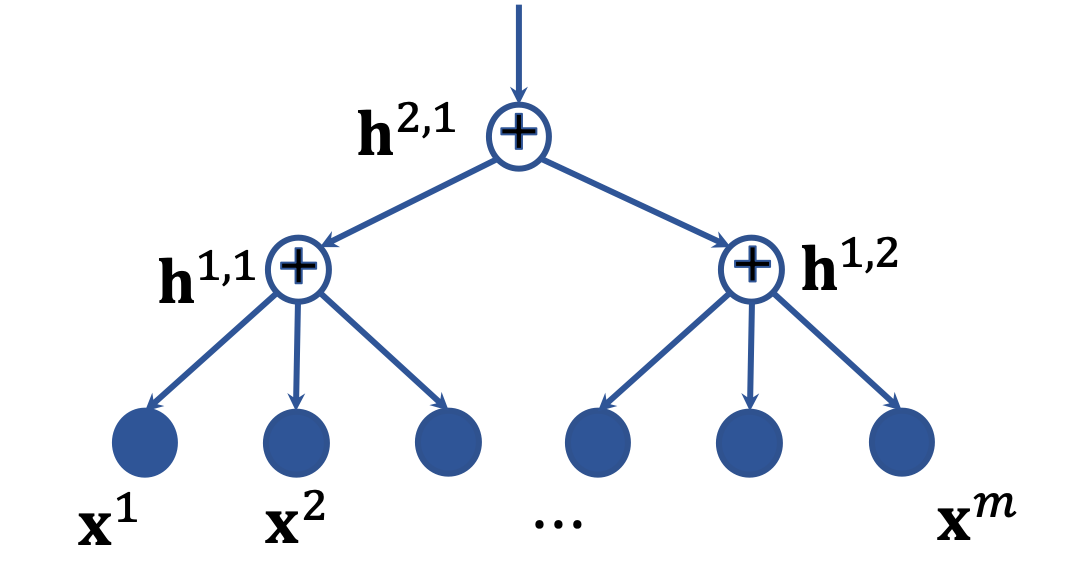
\includegraphics[width=2.3in]{fig/tree_direct.png}
    \caption{Tree structure.}
    \label{fig:tree-d}
\end{figure}

With the flow-based ensemble model, each edge is invertible.   The hierarchy of recognition network is the procedure from top to down of the structure as shown in Figure~\ref{fig:tree-d}.  Similarly, with the Markov property of the structure, the posterior density of the latent 
variables is given by
\begin{align*}
q(\mathbf{h}| \mathbf{x}, \theta ) = q(\mathbf{h}^1 | \mathbf{x}, \theta)  q(\mathbf{h}^2 | \mathbf{h}^1, \theta) \cdot \cdot  \cdot  q(\mathbf{h}^{L} | \mathbf{h}^{L-1}, \theta) .
\end{align*}
It can be simplified as 
\begin{align*}
q(\mathbf{h}| \mathbf{x}) = q(\mathbf{h}^1 | \mathbf{x})  q(\mathbf{h}^2 | \mathbf{h}^1) \cdot \cdot  \cdot  q(\mathbf{h}^{L} | \mathbf{h}^{L-1}) .
\end{align*}
We also have 
\begin{align} \label{eq:chain}
q(\mathbf{h}| \mathbf{x}) = q(\mathbf{h}^1 | \mathbf{x})  q(\mathbf{h}^{2:L} | \mathbf{h}^1) .
\end{align}

To derive the ELBO of a hierarchy model, we take all  layers of latent variables as the latent vector in conventional VAE, and we have 
\begin{align*}
&\log p(\mathbf{x})\\
=&  \mathbb{E}_{q(\mathbf{h} | \mathbf{x})} \bigg[ \log  \frac{p(\mathbf{x}, \mathbf{h})}{p(\mathbf{h}|\mathbf{x})} \bigg] \\
=&  \mathbb{E}_{q(\mathbf{h} | \mathbf{x})} \bigg[ \log  \frac{p(\mathbf{x}, \mathbf{h})}{q(\mathbf{h}|\mathbf{x})}   \frac{q(\mathbf{x}, \mathbf{h})}{p(\mathbf{h}|\mathbf{x})} \bigg] \\
=&  \underbrace{\mathbb{E}_{q(\mathbf{h} | \mathbf{x})} \bigg[ \log  \frac{p(\mathbf{x}, \mathbf{h})}{q(\mathbf{h}|\mathbf{x})}  \bigg]}_{\underset{\text{(ELBO)}}{\mathcal{L}_{\theta}(x)}} +   \underbrace{\mathbb{E}_{q(\mathbf{h} | \mathbf{x})} \bigg[ \log \frac{q(\mathbf{h} |\mathbf{x})}{p(\mathbf{h}|\mathbf{x})} \bigg]}_{\text{KL}\big(q(\mathbf{h} |\mathbf{x}) | p(\mathbf{h}|\mathbf{x})\big)} .
\end{align*}
With $\text{KL}\big(q(\mathbf{h} |\mathbf{x}) | p(\mathbf{h}|\mathbf{x})\big) \geq 0$, we have 

\begin{align}  \label{eq:tree_elbo}
&\log p(\mathbf{x})  \geq  \mathcal{L}_{\theta}(x) \\  \notag
=&  \mathbb{E}_{q(\mathbf{h} | \mathbf{x})} \bigg[ \log  \frac{p(\mathbf{x}, \mathbf{h})}{q(\mathbf{h}|\mathbf{x})}  \bigg]  \\  \notag
=&  \mathbb{E}_{q(\mathbf{h}^{1:L} | \mathbf{x})} \bigg[ \log  \frac{p(\mathbf{x} | \mathbf{h}^{1:L}) p( \mathbf{h}^{1:L})}{q(\mathbf{h}^{1:L}|\mathbf{x})}  \bigg]  \\   \notag
 =&  \mathbb{E}_{q(\mathbf{h}^{1:L} | \mathbf{x})} \bigg[  \log p(\mathbf{x} | \mathbf{h}^{1:L})  \bigg]  +  \mathbb{E}_{q(\mathbf{h}^{1:L} | \mathbf{x})} \bigg[ \log   \frac{p( \mathbf{h}^{1:L})}{q(\mathbf{h}^{1:L}|\mathbf{x})}  \bigg]   \\    \label{eq:layer0_a}
=&  \mathbb{E}_{q(\mathbf{h}^{1:L} | \mathbf{x})} \bigg[ \log p(\mathbf{x} | \mathbf{h}^{1})  \bigg]  +  \mathbb{E}_{q(\mathbf{h}^{1:L} | \mathbf{x})} \bigg[ \log     \frac{p( \mathbf{h}^{1:L})}{q(\mathbf{h}^{1:L}|\mathbf{x})}  \bigg]  \\ 
=&  \underbrace{ \mathbb{E}_{q(\mathbf{h}^{1} | \mathbf{x})} \bigg[ \log  p(\mathbf{x} | \mathbf{h}^{1})  \bigg] }_{  \parbox{10.5em}{Reconstruction of the data given hidden layer 1}}  +  \underbrace{  \mathbb{E}_{q(\mathbf{h}^{1:L} | \mathbf{x})} \bigg[ \log  \frac{p( \mathbf{h}^{1:L})}{q(\mathbf{h}^{1:L}|\mathbf{x})}  \bigg] }_{-\text{KL}^{1:L}}.     \label{eq:layer0_b}
\end{align}

The first term in~\eqref{eq:layer0_a} is due to $p(\mathbf{x}|\mathbf{h}^{1:L}) =  p(\mathbf{x}|\mathbf{h}^{1})$. The first term in~\eqref{eq:layer0_b} is due to that the expectation is regarding $\mathbf{h}^{1}$. The hidden variables $\mathbf{h}^{l+1:L}$ can be taken as the parameters for $\mathbf{h}^l$'s  prior distribution .  We expand the minus KL term in~\eqref{eq:layer0_b} as follows
\begin{align} \label{eq:kl_1}
&-\text{KL}^{1:L} \\ \notag
=& \mathbb{E}_{q(\mathbf{h}^{1:L} | \mathbf{x})} \bigg[ \log  \frac{p( \mathbf{h}^{1:L})}{q(\mathbf{h}^{1:L}|\mathbf{x})}  \bigg]   \\ \notag
= &   \mathbb{E}_{q(\mathbf{h}^{1:L} | \mathbf{x})} \bigg[ \log  \frac{p( \mathbf{h}^{1}|  \mathbf{h}^{2:L}) p( \mathbf{h}^{2:L})  }{\underbrace{ q(\mathbf{h}^{1}|\mathbf{x}) q(\mathbf{h}^{2:L}|\mathbf{h}^1)}_{\text{Due to}~\eqref{eq:chain}} }  \bigg] \\ \notag
=&  \underbrace{  \mathbb{E}_{q(\mathbf{h}^{1:L} | \mathbf{x})} \bigg[ \log  \frac{p( \mathbf{h}^{1}|  \mathbf{h}^{2:L}) p( \mathbf{h}^{2:L})  }{ q(\mathbf{h}^{2:L}|\mathbf{h}^1)}  \bigg]  }_{(a)} +   \underbrace{\mathbb{E}_{q(\mathbf{h}^{1:L} | \mathbf{x})} \bigg[ \log \frac{1}{q(\mathbf{h}^{1}|\mathbf{x}) } \bigg] }_{(b)}  \notag
\end{align}

Given a batch of data, we take the inference in each layer as encoding and decoding procedures. In forward message passing, the hidden layer $\mathbf{h}^l$  only depends on its previous layer $l-1$. 
The logarithm term in (a) only relates to hidden states $\mathbf{h}^{1:L}$.  With the feed message from the child layer $\overrightarrow{\mathbf{h}}^{(i)}$ and the reconstruct message $\overleftarrow{\mathbf{h}}^{(i)}$  from the parent layer, we can derive the ELBO term for the likelihood of  $\overrightarrow{\mathbf{h}}^{(i)}$ .  With~\eqref{eq:chain}, given the hidden states $\mathbf{h}^1$ samples from layer 0, we have 
\begin{align} \label{eq:kl_a}
(a)  &=   \mathbb{E}_{q(\mathbf{h}^{1}|\mathbf{x})} \bigg[  \mathbb{E}_{q(\mathbf{h}^{2:L}|\mathbf{h}^1)} \bigg[ \log  \frac{p( \mathbf{h}^{1}|  \mathbf{h}^{2:L}) p( \mathbf{h}^{2:L})  }{ q(\mathbf{h}^{2:L}|\mathbf{h}^1)}  \bigg]    \bigg] .
\end{align}
The inner expectation is actually the ELBO for layer hidden variable $\mathbf{h}^1$. Hence
\begin{align} \notag
 &\mathbb{E}_{q(\mathbf{h}^{2:L}|\mathbf{h}^1)} \bigg[ \log  \frac{p( \mathbf{h}^{1}|  \mathbf{h}^{2:L}) p( \mathbf{h}^{2:L})  }{ q(\mathbf{h}^{2:L}|\mathbf{h}^1)}  \bigg]   \\ \notag
 =&\mathbb{E}_{q(\mathbf{h}^{2:L}|\mathbf{h}^1)} \big[  p( \mathbf{h}^{1}|  \mathbf{h}^{2:L})    \big] + \mathbb{E}_{q(\mathbf{h}^{2:L}|\mathbf{h}^1)} \bigg[ \log  \frac{ p( \mathbf{h}^{2:L})   }{ q(\mathbf{h}^{2:L}|\mathbf{h}^1)}  \bigg]  \\  \label{eq:a_inner}
 =&  \mathbb{E}_{q(\mathbf{h}^{2}|\mathbf{h}^1)} \big[  p( \mathbf{h}^{1}|  \mathbf{h}^{2})    \big] + \mathbb{E}_{q(\mathbf{h}^{2:L}|\mathbf{h}^1)} \bigg[ \log  \frac{ p( \mathbf{h}^{2:L})   }{ q(\mathbf{h}^{2:L}|\mathbf{h}^1)}  \bigg] \\ \notag
  =&  \mathbb{E}_{q(\mathbf{h}^{2}|\mathbf{h}^1)} \big[  p( \mathbf{h}^{1}|  \mathbf{h}^{2})    \big] - \text{KL}^{2:L} .
\end{align}

For the term (b),
\begin{align} \notag
 (b) & = \mathbb{E}_{q(\mathbf{h}^{1:L} | \mathbf{x})} \bigg[ \log \frac{1}{q(\mathbf{h}^{1}|\mathbf{x}) } \bigg] \\ \notag
&=  \mathbb{E}_{q(\mathbf{h}^{1} | \mathbf{x})} \bigg[ \log \frac{1}{q(\mathbf{h}^{1}|\mathbf{x}) } \bigg] \\ \label{eq:kl_b}
& = \text{H}(\mathbf{h}^{1}|\mathbf{x}) .
\end{align}

With~\eqref{eq:kl_1}~\eqref{eq:kl_a}~\eqref{eq:a_inner}~\eqref{eq:kl_b}, 
\begin{align*}
&-\text{KL}^{1:L} = \\
&    \mathbb{E}_{q(\mathbf{h}^{1}|\mathbf{x})} \bigg[  \mathbb{E}_{q(\mathbf{h}^{2}|\mathbf{h}^1)} \big[  p( \mathbf{h}^{1}|  \mathbf{h}^{2})    \big]  - \text{KL}^{2:L}  \bigg] +  \text{H}_q(\mathbf{h}^{1}|\mathbf{x}).
\end{align*}

Similarly, for layer $l$, we  have 
\begin{align*} % \label{eq:KL_l}
-\text{KL}^{l:L} 
=  & \mathbb{E}_{q(\mathbf{h}^{l}|\mathbf{h}^{l-1})} \bigg[  \mathbb{E}_{q(\mathbf{h}^{l+1}|\mathbf{h}^l)} \big[  p( \mathbf{h}^{l}|  \mathbf{h}^{l+1})    \big]  - \text{KL}^{l+1:L}  \bigg] \\ \notag
& +  \text{H}_q(\mathbf{h}^{l}|\mathbf{h}^{l-1}) \\ \notag
=&    \mathbb{E}_{q(\mathbf{h}^{l}|\mathbf{h}^{l-1})} \bigg[  \mathbb{E}_{q(\mathbf{h}^{l+1}|\mathbf{h}^l)} \big[  p( \mathbf{h}^{l}|  \mathbf{h}^{l+1})    \big]   \bigg] +  \text{H}_q(\mathbf{h}^{l}|\mathbf{h}^{l-1}) \\ \notag
& - \text{KL}^{l+1:L}.
\end{align*}

%Given a batch of samples, we compute the latent structure layer by layer.\textcolor{red}{ Need a figure to illustrate the computation.}
Given a batch of samples, we compute  and store the forward message and the backward message for each node in the forward and backward message passing procedures.  The above KL term can be simplified as
\begin{align} \label{eq:KL_tree}
-\text{KL}^{l:L} 
=&     \mathbb{E}_{q(\mathbf{h}^{l+1}|\mathbf{h}^l)} \big[  p( \mathbf{h}^{l}|  \mathbf{h}^{l+1})    \big]  +  \text{H}_q(\mathbf{h}^{l}|\mathbf{h}^{l-1}) \\ \notag
& - \text{KL}^{l+1:L}.
\end{align}



For a hierarchy model with $L$ layers, we can recursively expand the KL term regarding the ELBO for each layer.  Thus 
\begin{align} \label{eq:KL_all}
& \mathbb{E}_{q(\mathbf{h}^{1:L} | \mathbf{x})} \bigg[ \log  \frac{p( \mathbf{h}^{1:L})}{q(\mathbf{h}^{1:L}|\mathbf{x})}  \bigg] \\ \notag
=& \sum_{l=1}^{L-1} \bigg\{   \mathbb{E}_{q(\mathbf{h}^{l+1}|\mathbf{h}^l)} \bigg[ \log p( \mathbf{h}^{l}|  \mathbf{h}^{l+1})   \bigg]  +    \text{H}(\mathbf{h}^l | \mathbf{h}^{l-1} )  \bigg\}\\ \notag
&+  \mathbb{E}_{q(\mathbf{h}^L|\mathbf{h}^{L-1})} \bigg[ \log p( \mathbf{h}^{L-1}|  \mathbf{h}^L) )  \bigg]   \\ \notag
&-   \text{KL}\big(q(\mathbf{h}^L | \mathbf{h}^{L-1} )   | p(\mathbf{h}^L)  \big)
 \end{align}
%=&  \sum_{l=1}^{L-1} \bigg\{   \mathbb{E}_{q(\mathbf{h}^{l+1}|\mathbf{h}^l)} \bigg[ \log p( \mathbf{h}^{l}|  \mathbf{h}^{l+1})   \bigg]  +    \text{H}(\mathbf{h}^l | \mathbf{h}^{l-1} )  \bigg\}\\
%&+  \mathbb{E}_{q(\mathbf{h}^L|\mathbf{h}^{L-1})} \bigg[ \log p( \mathbf{h}^{L-1}|  \mathbf{h}^L)   p( \mathbf{h}^L)  \bigg] \\
%& +    \text{H}(\mathbf{h}^L | \mathbf{h}^{L-1} )  \\

With $\mathbf{h}^0 = \mathbf{x}$,  with the ELBO can be written as 
\begin{align*}
\log p(\mathbf{x}) \geq &   \sum_{l=0}^{L-1}  \mathbb{E}_{q(\mathbf{h}^{l+1}|\mathbf{h}^l)} \bigg[ \log p( \mathbf{h}^{l}|  \mathbf{h}^{l+1})   \bigg] + \\
& \sum_{l=1}^{L-1}   \text{H}_q(\mathbf{h}^l | \mathbf{h}^{l-1} ) -   \text{KL}\big(q(\mathbf{h}^L | \mathbf{h}^{L-1} )   | p(\mathbf{h}^L)  \big) . 
 \end{align*}
%For vanilla VAE models, $L=1$, $\mathbf{h}^0 = \mathbf{x}$, and $\mathbf{h}^1 = \mathbf{z}$. %, and $\mathbf{h}^2 = (\mu_{\mathbf{z}}, \sigma_{\mathbf{z}})$

\section*{Appendix B.  ELBO of DAG Models}\label{appd:dag_elbo}

If we reverse the edge directions in a DAG, the  result graph is still a DAG graph.  The nodes can be listed in a topological order regarding the DAG structure as shown in Figure~\ref{fig:dag}. By taking the topology order as the layers in tree structures, we can derive the ELBO for DAG structures.  Let's assume the DAG structure has $L$ layers, and the root nodes are in layer $L$. With $\mathbf{h}$ to represent the whole latent variables, following~\eqref{eq:tree_elbo} we have the ELBO for the log-likelihood of  data 
\begin{align}  \label{eq:dag_elbo}
&\log p(\mathbf{x})  \geq  \mathcal{L}_{\theta}(x)  \\ \notag
 =&  \mathbb{E}_{q(\mathbf{h} | \mathbf{x})} \bigg[ \log  \frac{p(\mathbf{x}, \mathbf{h})}{q(\mathbf{h}|\mathbf{x})}  \bigg]  \\ \notag
=&  \underbrace{ \mathbb{E}_{q(\mathbf{h}^{pa(\mathbf{x})} | \mathbf{x})} \bigg[ \log  p(\mathbf{x} | \mathbf{h}^{pa(\mathbf{x})})  \bigg] }_{  \parbox{10.5em}{Reconstruction of the data given the parent nodes of the data}}  +  \underbrace{  \mathbb{E}_{q(\mathbf{h}| \mathbf{x})} \bigg[ \log  \frac{p( \mathbf{h})}{q(\mathbf{h}|\mathbf{x})}  \bigg] }_{-\text{KL}}.   \notag
\end{align}

\begin{figure}[!htbp]
    \centering
    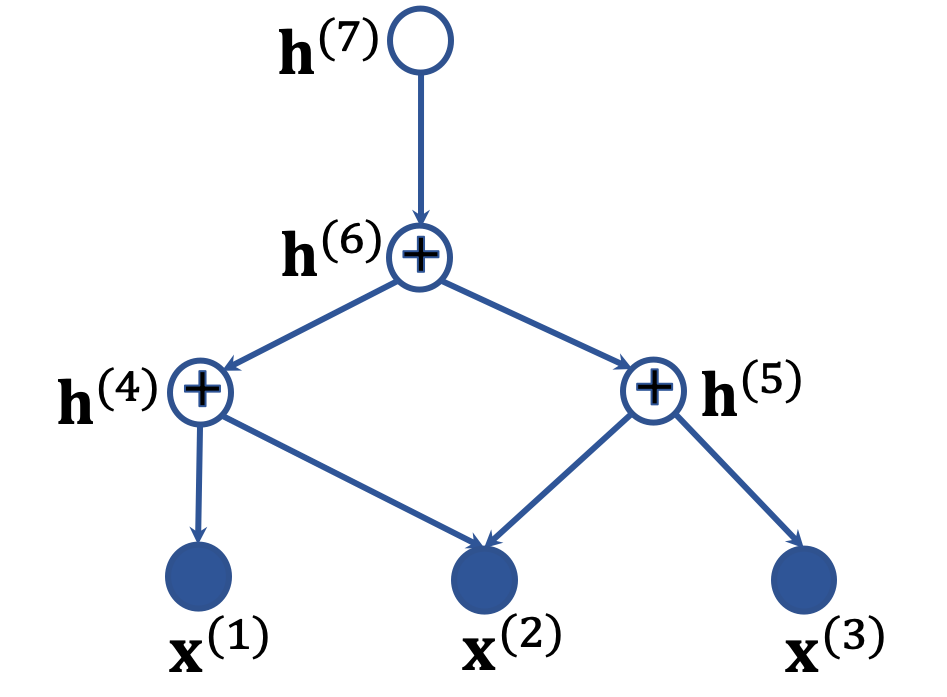
\includegraphics[width=2.3in]{fig/dag.png}
    \caption{DAG structure. The inverse topology order is \big\{ \{1,2,3\}, \{4,5\}, \{6\},  \{7\} \big\}, and it corresponds to layers 0 to 3.  }
    \label{fig:dag}
\end{figure}

Similarly the KL term can be expanded as in the tree structures. For nodes in layer $l$
\begin{align} \label{eq:KL_dag1}
-\text{KL}^{l:L} 
=&     \mathbb{E}_{q(\mathbf{h}^{pa(l)}|\mathbf{h}^l)} \big[  p( \mathbf{h}^{l}|  \mathbf{h}^{pa(l)})    \big]  +  \text{H}_q(\mathbf{h}^{l}|\mathbf{h}^{ch(l)}) \\ \notag
& - \text{KL}^{l+1:L}.
\end{align}
The forward and backward messages or latent state of a node are stored in the message passing procedures. They can be used by the node's parents and children  to compute the ELBO.  
It enables the calculation even the parents or children are  not  in layer~$l+1$ or $l-1$. For the node $i$ in layer $l$,   $pa(i)$ may have children in layers below $l$. Some nodes in $l$ may not have parent, and combining with the prior, the entropy term will become an KL term in this case.  Thus,  we have 
\begin{align} \label{eq:KL_dag2}
&-\text{KL}^{l:L} \\ \notag
=&   \sum_{i:i\in l, i \not\in   \mathcal{R}_{ \mathcal{G}} }  \bigg\{ \mathbb{E}_{q(\mathbf{h}^{pa(i)}|\mathbf{h}^{ch(pa(i))}} \big[  p( \mathbf{h}^{i}|  \mathbf{h}^{pa(i)})    \big]   +  \text{H}_q(\mathbf{h}^{i}|\mathbf{h}^{ch(i)})  \bigg\}  \\ \notag
& -  \sum_{i \in l \bigcap \mathcal{R}_{ \mathcal{G} }  }  \text{KL}\big(q(\mathbf{h}^{(i)} | \mathbf{h}^{ch(i)} )   | p(\mathbf{h}^{(i)})  \big)  - \text{KL}^{l+1:L}. \notag
\end{align}

By recurrently applying~\eqref{eq:KL_dag2}, we have 
\begin{align} \label{eq:kl_dag3}
& \mathbb{E}_{q(\mathbf{h} | \mathbf{x})} \bigg[ \log  \frac{p( \mathbf{h})}{q(\mathbf{h}|\mathbf{x})}  \bigg] \\ \notag
=& \sum_{l=1}^{L-1}   \sum_{i:i\in l, i \not\in   \mathcal{R}_{ \mathcal{G}}  }  \bigg\{ \mathbb{E}_{q(\mathbf{h}^{pa(i)}|\mathbf{h}^{(i)})} \bigg[ \log p( \mathbf{h}^{(i)}|  \mathbf{h}^{pa(i)})   \bigg] \\
& +    \text{H}(\mathbf{h}^i | \mathbf{h}^{ch(i)} )  \bigg\} \notag
 -   \sum_{l=1}^{L-1}  \sum_{i \in l \bigcap \mathcal{R}_{ \mathcal{G} }  }  \text{KL}\big(q(\mathbf{h}^{(i)} | \mathbf{h}^{ch(i)} )   | p(\mathbf{h}^{(i)})  \big) \\
 & -   \text{KL}\big(q(\mathbf{h}^L | \mathbf{h}^{L-1} )   | p(\mathbf{h}^L)  \big)   
 \end{align}
Since $L  \subseteq   \mathcal{R}_{ \mathcal{G}} $,  with $\mathbf{h}^{(0)} = \mathbf{x}$,~\eqref{eq:dag_elbo}, and~\eqref{eq:kl_dag3} we have 
\begin{align*}  
& \log p(\mathbf{x}) \geqslant \mathcal{L}(\mathbf{x}; \theta) \\
=&   \sum_{i \in \mathcal{G}  \setminus  \mathcal{R}_{ \mathcal{G} }  }  \mathbb{E}_{q(\mathbf{h}^{pa(i)}|\mathbf{h}^{ch(pa(i))})} \bigg[ \log p( \mathbf{h}^{(i)}|  \mathbf{h}^{pa(i)})   \bigg]  \\
 & +  \sum_{i \in \mathcal{G}  \setminus  \mathcal{R}_{ \mathcal{G} }  } H_q(\mathbf{h}^{(i)} | \mathbf{h}^{ch(i)} )   -    \sum_{i \in  \mathcal{R}_{ \mathcal{G} }  }  \text{KL}\big(q(\mathbf{h}^{(i)} | \mathbf{h}^{ch(i)} )   | p(\mathbf{h}^{(i)})  \big) .   
 \end{align*}

 
\section*{Appendix D.  Structure Recovery }


\end{document}
